%%%%%%%%%%%%%%%%%%%%%%%%%%%%%%%%%%%%%%%%%%%%%%%%%%%%%%%%%%%%%%%%%%%%%%%%
%    INSTITUTE OF PHYSICS PUBLISHING                                   %
%                                                                      %
%   `Preparing an article for publication in an Institute of Physics   %
%    Publishing journal using LaTeX'                                   %
%                                                                      %
%    LaTeX source code `ioplau2e.tex' used to generate `author         %
%    guidelines', the documentation explaining and demonstrating use   %
%    of the Institute of Physics Publishing LaTeX preprint files       %
%    `iopart.cls, iopart12.clo and iopart10.clo'.                      %
%                                                                      %
%    `ioplau2e.tex' itself uses LaTeX with `iopart.cls'                %
%                                                                      %
%%%%%%%%%%%%%%%%%%%%%%%%%%%%%%%%%%
%
%
% First we have a character check
%
% ! exclamation mark    " double quote  
% # hash                ` opening quote (grave)
% & ampersand           ' closing quote (acute)
% $ dollar              % percent       
% ( open parenthesis    ) close paren.  
% - hyphen              = equals sign
% | vertical bar        ~ tilde         
% @ at sign             _ underscore
% { open curly brace    } close curly   
% [ open square         ] close square bracket
% + plus sign           ; semi-colon    
% * asterisk            : colon
% < open angle bracket  > close angle   
% , comma               . full stop
% ? question mark       / forward slash 
% \ backslash           ^ circumflex
%
% ABCDEFGHIJKLMNOPQRSTUVWXYZ 
% abcdefghijklmnopqrstuvwxyz 
% 1234567890
%
%%%%%%%%%%%%%%%%%%%%%%%%%%%%%%%%%%%%%%%%%%%%%%%%%%%%%%%%%%%%%%%%%%%
%
\documentclass[12pt]{iopart}
\bibliographystyle{iopart-num_custom}
\usepackage{xcolor}
\usepackage{pifont}
\usepackage{comment}
\usepackage{acronym}
\usepackage{standalone}
\usepackage{academicons}
\usepackage{scalerel}
\usepackage{layouts}
\usepackage{import}
%\usepackage{subfig}
\usepackage{subcaption}
\usepackage{tikz}
\usetikzlibrary{decorations.pathreplacing,angles,quotes,shapes.geometric, arrows,calc}
\usetikzlibrary{svg.path}
\expandafter\let\csname equation*\endcsname\relax 
\expandafter\let\csname endequation*\endcsname\relax 
\usepackage{amsmath}
\usepackage{amssymb}
\usepackage{hyperref}
\usepackage{bibentry}
\usepackage[capitalize]{cleveref}


\usepackage{graphicx}
\usetikzlibrary{decorations.pathreplacing,angles,quotes,shapes.geometric, arrows,calc}
\usepackage{wrapfig, blindtext}
\usepackage{pgfplots}
\pgfplotsset{compat=1.16}

\usepackage[mathlines]{lineno}% Enable numbering of text and display math
\linenumbers\relax % Commence numbering lines

% Commands for references
\def\prd{\ref@jnl{Phys.~Rev.~D}}

\newcommand{\gguide}{{\it Preparing graphics for IOP Publishing journals}}
%Uncomment next line if AMS fonts required
%\usepackage{iopams}  
\newcommand{\jordan}[1]{\textbf{\textcolor{red}{JORDAN: #1}}}
\newcommand{\siong}[1]{\textbf{\textcolor{blue}{SIONG: #1}}}
\newcommand{\chris}[1]{\textbf{\textcolor{green}{CHRIS: #1}}}
\newcommand{\michael}[1]{\textbf{\textcolor{orange}{MICHAEL: #1}}}
\newcommand{\dcc}{LIGO-PXXXXXXX}

\newcommand{\ndimensional}[1]{$#1$\nobreakdash\discretionary{-}{-}{-}dimensional}

%\input{tag.tex}
% Command for ORCID id's
\definecolor{orcidlogocol}{HTML}{A6CE39}
\tikzset{
  orcidlogo/.pic={
    \fill[orcidlogocol] svg{M256,128c0,70.7-57.3,128-128,128C57.3,256,0,198.7,0,128C0,57.3,57.3,0,128,0C198.7,0,256,57.3,256,128z};
    \fill[white] svg{M86.3,186.2H70.9V79.1h15.4v48.4V186.2z}
                 svg{M108.9,79.1h41.6c39.6,0,57,28.3,57,53.6c0,27.5-21.5,53.6-56.8,53.6h-41.8V79.1z M124.3,172.4h24.5c34.9,0,42.9-26.5,42.9-39.7c0-21.5-13.7-39.7-43.7-39.7h-23.7V172.4z}
                 svg{M88.7,56.8c0,5.5-4.5,10.1-10.1,10.1c-5.6,0-10.1-4.6-10.1-10.1c0-5.6,4.5-10.1,10.1-10.1C84.2,46.7,88.7,51.3,88.7,56.8z};
  }
}

\newcommand\orcidicon[1]{\href{https://orcid.org/#1}{\mbox{\scalerel*{
\begin{tikzpicture}[yscale=-1,transform shape]
\pic{orcidlogo};
\end{tikzpicture}
}{|}}}}

\usepackage{hyperref} %<--- Load after everything else

\begin{document}

\title{Generalised gravitational burst generation with Generative Adversarial Networks}

\author{
    J. McGinn \orcidicon{0000-0000-0000-0000},
    C. Messenger \orcidicon{0000-0001-7488-5022},
    I.S. Heng \orcidicon{0000-0000-0000-0000},
    M. J. Williams \orcidicon{0000-0003-2198-2974}
}

\address{University of Glasgow, Physics \& Astronomy Department, Glasgow G12 8QQ, UK}
%\ead{jordan.mcginn@glasgow.ac.uk}
\vspace{10pt}
%\begin{indented}
%\item[]\commitDATE\\\mbox{\small \commitID}\\\mbox{\dcc}
%\end{indented}

\begin{abstract}
We introduce the use of conditional generative adversarial networks for generalised gravitational wave burst generations in the time domain. Generative adversarial networks are generative machine learning models that produce new data based on the statistics of the training set. We condition the network on five classes of time-series signals: sine-Gaussian, ringdown, white noise burst, Gaussian pulse and binary black hole merger and show that the model can replicate the features of these classes. Additionally, we show the model can produce generalised burst signals through interpolation and class mixing. Further, we build a convolution neural network classifier to predict the detectability of these newly produced signals in LIGO detector noise against more traditional burst waveforms. 
\end{abstract}

%
% Uncomment for keywords
%\vspace{2pc}
%\noindent{\it Keywords}: XXXXXX, YYYYYYYY, ZZZZZZZZZ
%
% Uncomment for Submitted to journal title message
%\submitto{\JPA}
%
% Uncomment if a separate title page is required
%\maketitle
% 
% For two-column output uncomment the next line and choose [10pt] rather than [12pt] in the \documentclass declaration
%\ioptwocol
%

\acrodef{GW}[GW]{gravitational wave}
\acrodef{CBC}[CBC]{compact binary coalescence} 
\acrodef{ML}[ML]{machine learning}
\acrodef{AI}[AI]{artificial intelligence}
\acrodef{CNN}[CNN]{convolutional neural network}
\acrodef{GAN}[GAN]{generative adversarial network}
\acrodef{CGAN}[CGAN]{conditional generative adversarial network}
\acrodef{ACGAN}[ACGAN]{auxilliary conditional generative adversarial network}
\acrodef{DCGAN}[DCGAN]{deep convolutional generative adversarial network}
\acrodef{CNN}[CNN]{convolutional neural networks}
\acrodef{BBH}[BBH]{binary black hole}
\acrodef{SNR}[SNR]{signal-to-noise ratio}
\acrodef{PSD}[PSD]{power spectral density}


%%%%%%%%%%%%%%%%%%%%%%%%%%%%%%%%%%%%%%%%%%%%%%%%%%%%%%%%%%%%%%%%%%%%%%%%%%%%%%
%%%%%%%%%%%%%%%%%%%%%%%%%%%%%%%%%%%%%%%%%%%%%%%%%%%%%%%%%%%%%%%%%%%%%%%%%%%%%%
\section{Introduction}
%%%%%%%%%%%%%%%%%%%%%%%%%%%%%%%%%%%%%%%%%%%%%%%%%%%%%%%%%%%%%%%%%%%%%%%%%%%%%%
%%%%%%%%%%%%%%%%%%%%%%%%%%%%%%%%%%%%%%%%%%%%%%%%%%%%%%%%%%%%%%%%%%%%%%%%%%%%%%
%textwidth in inches: \printinunitsof{in}\prntlen{\textwidth}
\begin{comment}
\begin{itemize}
\item Need to introduce GWs - the current state of the field e.g. detections
and LVC papers \ding{51}
\item Introduce burst searches - what's the point of burst searches \ding{51} - lots of references 
\item Discuss the family of burst waveforms currently used and why - not in detail, just
an introduction \ding{51}
\item Introduce ML techniques in GWs \ding{51} - lots of references
\item What this paper does on GANs in 1 paragraph \ding{51}
\item Describe the structure of the paper 
\end{itemize}
\end{comment}

% introduce \ac{GW} astrophsyics
%
Gravitational wave astronomy is now an established field that began with the first
detection of a binary black hole merger~\cite{Abbott2016} in September 2015.
Following this, the first and second observations runs (O1 and O2) of Advanced
LIGO and Advanced Virgo~\cite{Prospects-dets, AdvLIGO, AdvLIGO2, AdvVIRGO}
reported several more \ac{CBC} mergers~\cite{Abbott2016a, Abbott2017,
Abbott2017a, Abbott2017b}. On 17th August 2017 a binary neutron star merger was
observed alongside its electromagnetic counterpart for the first time, giving
rise to multi-messenger \ac{GW} astronomy. 

% introduce burst searches
%
With these successes and continued upgrades to the detectors, further
detections of \acp{CBC} are expected to be commonplace in future advanced
detcetor observation runs. Another group of \ac{GW} signals that has thus far
been undetected is \ac{GW} ``bursts". \ac{GW} bursts are classed as transient
signals of typically short duration ($<$ 1s) whose waveforms are not accurately
modelled or are complex to reproduce. Astrophysical sources for such transients
include: Core collapse supernova~\cite{Fryer_2003}, Pulsar
glitches~\cite{Andersson_2001}, Neutron star post-mergers~\cite{Baiotti_2007}
and other as-yet unexplained astrophysical phenomena. 

% more details on burst searches
%
\ac{GW} searches for modelled signals use a process called
matched-filtering,~\cite{Owen1998,Usman_2016,sachdev2019gstlal}, where a large template bank of possible
\ac{GW} waveforms are compared to the detector outputs. For \ac{GW} bursts that remain unmodeled; there are no
templates available and so matched-filtering is unsuitable for the detection of
these signals.  Instead, detection algorithms like coherent WaveBurst \cite{drago2020coherent} involve distinguishing the signal from
detector noise by looking for excess power contained in the time-frequency
domain and rely on the
astrophysical burst waveform appearing in multiple detectors at similar times.
This is only possible if the detector noise is well characterised and the
candidate signal can be differentiated from systematic or environmental
glitches. 

% Discuss the family of burst waveforms currently used and why - not in detail, just
% an introduction 
%
\ac{GW} burst detection algorithms~\cite{Klimenko_2008, Aso_2008} are tested
and tuned using modelled waveforms that have easy to define parameters and share characteristics of real bursts that aim to simulate a \ac{GW} passing between
detectors. Such waveforms include sine-Gaussians: a
Gaussian modulated sine wave that is characterised by its central frequency and
decay parameter. Bandlimited white noise bursts: white noise that is contained
within a certain frequency range and ringdowns which mimic the damped
oscillations after a \ac{CBC} merger. A Gaussian pulse: a short exponential increase then decrease in amplitude and a binary black hole inspiral.
% cut this text if not going to be used
%
\begin{comment}Such waveforms may have
long-duration, short bandwidth (ringdowns), long-duration, large bandwidth
(inspirals) and many algorithms make use of sine-Gaussians: a Gaussian
modulated sine wave that is characterised by it's central frequency and narrow
bandwidth.~\chris{not the time to try to describe the types of burst waveforms.
Also, be careful with satying things like ringdowns have narrow bandwidth. I
know we specify a single frequency but becuase of the short duration, the
signal is broad band. Look at the FFT} This makes it a great tool for
diagnosing LIGOs sensitivity to frequency.~\chris{strange unfinished sentence.} 
\end{comment}

% Introduce ML techniques in GWs
%
With the expectation that there will be many more \ac{GW} detections in the
future, there is a growing need for fast and efficient \ac{GW} analysis methods
to match the rising number of detections. While still in its infancy, the application of \ac{ML} to \ac{GW} analyses has already shown great potential in areas of detection ~\cite{Gabbard2017,Gebhard_2019,Krastev_2020}, where these techniques have matched the sensitivity of matched filtering for Advanced LIGO and Advanced Virgo gravitational-wave searches. In identifying and classifying detector noise transients or  ``glitches''~\cite{Bahaadini, George_2018,Razzano_2018, 2020arXiv200801262G}. In Bayesian parameter
estimation~\cite{gabbard2019bayesian, green2020gravitationalwave} where \ac{ML} techniques can recover parameters of a \ac{GW} signal significantly faster than standard methods. Long duration signals like continuous \ac{GW} require long observing times and therefore have large amounts of data needing to be processed. Current \ac{ML} approaches~\cite{2020PhRvD.102b2005D, 2019PhRvD.100d4009D, 2020arXiv200708207B} are particularly well suited to dealing with this as once trained the searches can be performed quickly.

% What this paper does on GANs in 1 paragraph - the point of the paper
%
In this work we aim to explore the use of \ac{ML} to generate and interpret
unmodeled \ac{GW} burst waveforms. Using the generative machine learning
model, \acp{GAN}, we train on five classes of waveforms in the time domain. Working on the assumption that \acp{GAN} construct smooth
 high dimensional vector spaces between their input and output, we can then
explore the space between the five classes to construct new
hybrid waveforms. As all the computationally expensive
processes occur during training, once trained, the model is able to
generate waveforms in fractions of a second and produce waveforms that are difficult to generate with current
techniques. These new varieties of waveforms can then be used to diagnose \michael{not sure about diagnose, maybe test or evaluate?}
detection algorithms, gain new insight into sources of \ac{GW}
bursts and  allow us to better train our algorithms on a
broader range of possible signals and therefore enhance our detection ability. 

% the structure of the paper
%
This paper is organised as follows. In \cref{ML overview} we introduce the basic ideas of machine learning and discuss the choice of algorithm we used. In \cref{Method} we describe the training data and the details of the model. We present the results of the GAN in \cref{results} and show how unmodeled signals can be produced by interpolating and sampling within latent and class spaces. In \cref{cnn classifier} we show that a convolutional neural network \michael{should this have the accronym? Tried to fix it but it only puts the plural for me} classifier can be trained to distinguish between sets of our GAN generated waveforms from noise only cases. We conclude with a summary of the presented work in \cref{conclusions}.

%%%%%%%%%%%%%%%%%%%%%%%%%%%%%%%%%%%%%%%%%%%%%%%%%%%%%%%%%%%%%%%%%%%%%%%%%%%%%%
%%%%%%%%%%%%%%%%%%%%%%%%%%%%%%%%%%%%%%%%%%%%%%%%%%%%%%%%%%%%%%%%%%%%%%%%%%%%%%
\section{Machine learning} \label{ML overview}
%%%%%%%%%%%%%%%%%%%%%%%%%%%%%%%%%%%%%%%%%%%%%%%%%%%%%%%%%%%%%%%%%%%%%%%%%%%%%%
%%%%%%%%%%%%%%%%%%%%%%%%%%%%%%%%%%%%%%%%%%%%%%%%%%%%%%%%%%%%%%%%%%%%%%%%%%%%%%

\begin{comment}
\begin{itemize}
\item Describe GANs in detail but really focus on the fact that the reader is a
GW data analyst - not a computer scientist \ding{51}
\item A diagram would be very useful \ding{51}
\item Do not discuss our specific case here - just stay general \ding{51}
\item A subsection on the specific advanced flavour of GAN that you are using
here - motivate this choice. \ding{51}
\end{itemize}
\end{comment}

% introduce GANs
%
\subsection{Artificial neural networks}

% inroduce the concept of ML
%

\begin{figure}[h!]
\begin{subfigure}[b]{0.30\textwidth}
   \begin{subfigure}[b]{1\textwidth}
   	\centering
	\resizebox{\textwidth}{!}{
 	\begin{tikzpicture}		
		    \node[scale=0.3] 		   (x1) at (0,0.8) {$x_1$}; 
		    \node[scale=0.3] 		   (x2) at (0,0.5) {$x_2$};  
		    \node[scale=0.3] 		   (x3) at (0,0.2) {$x_3$};       
    		    \node [draw, circle,scale=0.18,fill=blue!25]          (c3) at (0.7,0.5) {\Large $\sigma(\sum_i w_i x_i + b)$};
    \draw[->] (x1)--(c3);
    \draw[->] (x2)--(c3);
    \draw[->] (x3)--(c3);
     \draw[->] (c3)--(1.3,0.5);
   	\end{tikzpicture}
	}
	\caption{}
	 \label{fig:perceptron}
 \end{subfigure}
 
   \begin{subfigure}[b]{1\textwidth}
  	\centering
	\resizebox{\textwidth}{!}{
\begin{tikzpicture}
\begin{axis}[
    xmin=-2.5, xmax=2.5,
    ymin=-1.5, ymax=1.5,
    axis lines=center,
    axis on top=true,
    domain=-2.5:2.5,
    ylabel=$\sigma$,
    xlabel=$x$,
    ]

    \addplot [mark=none,draw=purple,domain=-2.5:2.5,ultra thick] {1/(1+exp(-x))};
    \addplot+[mark=none,draw=green,domain=-2.5:0,ultra thick] {0};
    \addplot+[mark=none,draw=green,domain=0:2.5,ultra thick] {x};
    \addplot+[mark=none,orange,domain=-2.5:0,ultra thick] {0.2*x};
    \addplot+[mark=none,orange,domain=0:2.5,ultra thick] {x};

    %% Add the asymptotes
\end{axis}
\end{tikzpicture}
	}
	\caption{}
	 \label{fig:activations}
\end{subfigure}
\end{subfigure}
	 \begin{subfigure}[b]{0.70\textwidth}
\centering
\resizebox{\textwidth}{!}{
\def\layersep{1.5cm}
\begin{tikzpicture}[shorten >=1pt,draw=black, ->,node distance=\layersep]


    \tikzstyle{every pin edge}=[<-,shorten <=1pt]
    \tikzstyle{neuron}=[circle,draw=black, very thick, fill=blue!25, minimum size=22pt,inner sep=0pt]
    \tikzstyle{input neuron}=[circle,draw=black,very thick,fill=black!25, minimum size=22pt,inner sep=0pt];
    \tikzstyle{output neuron}=[neuron];
    \tikzstyle{hidden neuron}=[circle,draw=black,very thick,fill=blue!25,minimum size=22pt,inner sep=0pt];
    \tikzstyle{annot} = [text width=4em, text centered]

    % Draw the input layer nodes
    \foreach \name / \y in {1,...,5}
    % This is the same as writing \foreach \name / \y in {1/1,2/2,3/3,4/4}
        \node[input neuron] (I-\name) at (0,-\y) {$x_{\name}$};

    % Draw the hidden layer nodes
    \foreach \name / \y in {1,...,3}
        \path[yshift=-1cm]
            node[hidden neuron] (H-\name) at (\layersep,-\y cm) {};
            
  \foreach \namee / \y in {1,...,3}
        \path[yshift=-1 cm]
            node[hidden neuron] (H1-\namee) at (2*\layersep,-\y cm){};

           
    % Draw the output layer node
  \node[output neuron,pin={[pin edge={->}]right:}, right of=H1-2] (O) {};
    % Connect every node in the input layer with every node in the
    % hidden layer.
    \foreach \source in {1,...,5}
        \foreach \dest in {1,...,3}
            \path (I-\source) edge (H-\dest);

 \foreach \source in {1,...,3}
        \foreach \dest in {1,...,3}
            \path (H-\source) edge (H1-\dest);
            
    % Connect every node in the hidden layer with the output layer
    \foreach \source in {1,...,3}
        \path (H1-\source) edge (O);

    % Annotate the layers
    %\node[annot,above of=H-1, node distance=1cm] (hl) {Hidden layers};
   % \node[annot,left of=I-4] at (0) {Input layer};
    %\node[annot,right of=hl] {Output layer};
    
    \draw[decoration={brace,mirror,raise=15pt},decorate,-]
  (I-1.north) -- node[left=0.8cm,scale=0.7] {Input layer} (I-5.south);
 
    \draw[decoration={brace,raise=15pt},decorate,-]
  (H-1.west) --  node[above=0.8cm,scale=0.7]{Hidden layers}  (H1-1.east);
  
    \draw[decoration={brace,raise=15pt},decorate,-]
  (O.west) --  node[above=0.8cm,scale=0.7]{Output layers}  (O.east);
 
\end{tikzpicture}
}
 \caption{}
 \label{fig:network}
 \end{subfigure}

\caption{Neural Networks (a) A single neuron taking a vector of inputs and
returning a single output based on the weights, bias and activation function
of the network. (b) A selection of activation functions used in this study. The sigmoid (purple), rectified linear unit (ReLU) \cite{relu} (orange) and leaky rectified linear unit \cite{Maas2013RectifierNI} (green). (c)
A an example of a neural network containing two hidden layers that performs a
mapping of an input vector to a single output. \michael{Minor comment, it's hard to see what the ReLU is doing above 0, maybe use different line styles for each?}}
\end{figure}
%
% Introduce basic neural networks - a perceptron layer
%
\begin{comment}
Neural networks are the quintessential~\chris{really? quintessential?} \jordan{It's a perfectly cromulent word https://www.imdb.com/title/tt0701155/} \ac{ML}
algorithm that aims to approximate a function. 
\end{comment}

\ac{ML} algorithms aim to learn apparent relationships held within given data or `training
data' in order to make accurate predictions without the need for additional
programming. A common approach in \ac{ML} relies on the model learning from
past experience to make decisions on future events. Artificial neural networks are universal function approximators that are built from many single
processing units called neurons. The simplest neural network is the perceptron
layer~\cref{fig:perceptron} which shows a single neuron that takes a vector of real
inputs $x_{i},\ldots, x_{n}$
and maps them to an output according to the linear function, 
%
\begin{align}
f(x) = \sigma(\sum_i w_i x_i + b),
\label{eqn:neuron}
\end{align}
%
where $w$ and $b$ are the weights and bias and $\sigma$
denotes the activation function. The weights are numbers which can be thought
of as the strength between connected neurons. The output of a neuron is defined by its activation function which controls how the neuron `fires' depending on its input. Some examples of commonly used activation functions are shown in~\cref{fig:activations}. It is often useful to introduce a bias, $b$, such that the neuron remains inactive
above zero but is active when the sum reaches a defined threshold. 

% basic network structure
%
A neural network contains many single neurons connected in a layered structure
as shown in~\cref{fig:network}. The activations of the first layer (or
input layer) act as the inputs to the second layer and so on until the output
layer. Multi-layered neural networks have intermediate layers between the input
and output stages dubbed the hidden layers.
% the cost or loss function
%
The output of a single neuron is gives a
prediction that can be compared to the real value through a loss (also known as a
cost) function. The network is trained to minimise this function by updating the weights in the negative
direction of the loss gradient in a process referred to as gradient
descent \cite{ruder2016overview}. The training process for a single layered network is easy to compute as the weights relate directly to the gradient of the loss function the network is trying to minimise. For deeper architectures, the loss is a complicated function of all the weights in all the layers. The backpropagation \cite{Nielsen1992} algorithm acts over the many paths from node to output. It does so in two phases:

\begin{itemize}
\item Forward phase: For one instance of training, the inputs are fed forward through the network using the current weights and the final output is compared to the training labels. The derivative of the loss function is then computed.
\item Backward phase: This phase learns how the gradient of the loss function changes when the weights are varied. Starting at the output node, the algorithm goes backwards through the network (hence the name). The weights that give the steepest descent to the loss function are saved for the next training instance.  
\end{itemize}
This process of updating the weights is repeated until the loss function reaches convergence or a global minimum. As it is impractical to feed the entire data into the network at once, the training is split up into smaller more manageable batches. For this work we train on random samples from the training data and define an epoch as the number of training steps.


%%%%%%%%%%%%%%%%%%%%%%%%%%%%%%%%%%%%%%%%%%%%%%%%%%%%%%%%%%%%%%%%%%%%%%%%%%%%%%
\subsection{Convolutional Neural Networks}
%%%%%%%%%%%%%%%%%%%%%%%%%%%%%%%%%%%%%%%%%%%%%%%%%%%%%%%%%%%%%%%%%%%%%%%%%%%%%%
%
Convolutional neural networks (CNNs) are designed to work with grid-like input structures that exhibit
strong local spatial dependencies. Although most work with \acp{CNN}
involve image-based data, they can be applied to other spatially adjacent data
types such as time-series and text items. \acp{CNN} are defined by the use of a
convolution operation, a mathematical operation that expresses the amount
overlap between the data. Much like traditional neural networks the convolution operation in this context involves multiplying the input by an array of weights, called a filter or a kernel which is typically smaller in size than the input. The convolution is applied by shifting the kernel over the input, drawing out spatially important features between the
two. The distance by which the grid is shifted is known as
the stride and increasing it reduces the dimensionality of the output in a process know as downsampling. Alternatively, upsampling the inputs can be achieved using a transposed convolution \cite{dumoulin2016guide}. The output of the convolutional layer is then passed to an activation function and through the next layers. For deep neural networks, techniques like BatchNormalisation \cite{ioffe2015batch} which standardise the inputs to a layer and SpatialDropout \cite{tompson2014efficient} which sever connections between neurons can both help to stabilise learning.  


%%%%%%%%%%%%%%%%%%%%%%%%%%%%%%%%%%%%%%%%%%%%%%%%%%%%%%%%%%%%%%%%%%%%%%%%%%%%%%
\subsection{Generative Adversarial Networks}
%%%%%%%%%%%%%%%%%%%%%%%%%%%%%%%%%%%%%%%%%%%%%%%%%%%%%%%%%%%%%%%%%%%%%%%%%%%%%%
%
% basic intro to GANs
%
A subset of deep learning that has seen fruitful development in recent years
are generative adversarial networks \acp{GAN}~\cite{Goodfellow2014}. These unsupervised algorithms learn patterns in a
given training data set using an adversarial process. The generations from
\acp{GAN} are currently state-of-the-art in fields such as high quality image
fidelity~\cite{brock2018large,karras2019analyzing}, text-to-image
translation~\cite{reed2016generative}, and video
prediction~\cite{liang2017dual} as well as time series
generations~\cite{esteban2017realvalued}.
%
% Basic components of a GAN
%
\acp{GAN} train two competing neural networks, consisting of a discriminator
network that is set up to distinguish between real and fake data and a
generator network that produces fake versions of the real data. The generator model performs a mapping from a fixed length vector $\mathbf{z}$ to its
representation of the data. The input vector is drawn randomly from a Gaussian distribution which is referred to as a latent space comprised of latent variables. The latent space is a compressed representation of a data distribution which the generator applies meaning to during training. Sampling points from this space allows the generator to produce a variety of different generations, with different points corresponding to different features in the generations. The discriminator maps its input $\mathbf{x}$ to a probability that the input came from either the training (real) data or
generator (fake).
\begin{comment}
Chris' definition of latent space if needed: It maps the intrinsic
variation of the training space onto the Gaussian latent space distribution.
\end{comment}
%
% training a GAN
%
During training, the discriminator and generator are updated using batches of data. Random latent vectors are given to the generator to produce a batch of fake samples and an equal batch of real samples is taken from the training data. The discriminator makes predictions on the real and fake samples and the model is updated through minimising the binary cross-entropy function \cite{Goodfellow-et-al-2016}
%
\begin{equation}
    L = -y \log(\hat{y}) - (1 - y) \log(1-\hat{y}),
    \label{eqn:crossentropy}
\end{equation}
where $\hat{y}$ is the network prediction and $y$ is the true output. While training the discriminator, D, on real data, we set $y = 1$ and $\hat{y} = D(\mathbf{x})$ which from \cref{eqn:crossentropy} gives $L(D(\mathbf{x}),1) = \log(D(\mathbf{x}))$. While training on fake data produced by the generator, G, $y = 0$ and $\hat{y} = D(G(\mathbf{z}))$ and so, $L(D(G(\mathbf{z})),0) = \log(1-(D(G(\mathbf{z}))))$. Since the objective of the discriminator is to correctly classify fake and real data these equations should be maximised, while the goal of the generator should be to minimize these equations. This gives the \ac{GAN} loss as
%
\begin{equation}
   \mathop{\text{min}}_{G}  \mathop{\text{max}}_{D} V(D,G) = \mathbb{E}_{\mathbf{x} \sim p_{\text{\text{data}}}(\mathbf{x})} [\text{log} D(\mathbf{x})] + \mathbb{E}_{\mathbf{z} \sim p_{\mathbf{z}}(\mathbf{z})} [\text{log}(1-D(G(\mathbf{z})))],
 \label{equation:GANloss}
 \end{equation}
where $p_{\text{\text{data}}}(\mathbf{x})$ is the distribution of real data and $p_{\text{z}}(\mathbf{z})$ is the latent distribution. 

\subsection{Training stages}
%
Training a GAN is involves updating both the discriminator and generator in stages. First, the discriminator is updated on real instances from the training set. We set the true label $y=1$ and calculate the loss with respect to the predictions $\hat{y}$ via \cref{equation:GANloss}. Stochastic gradient descent is used to minimize the loss which has reduced to $L_D(\textrm{real}) = -\log(\hat{y})$. The discriminator is then trained on fake instances taken from the generator where we set $y=0$ and minimize $L_D(\textrm{fake}) = -\log(1-\hat{y})$. To train the generator, we use a composite model of the generator and discriminator and allow the gradients to flow through this entire model. At this step we set the labels for the generator as real $y=1$ and minimize $L_G = -\log(\hat{y})$. The act of switching the labels and minimizing this form of loss is identical to the previously mentioned generator loss but is beneficial as in practice this function provides more useful gradients. This tweak to the generator loss is called non-saturating generator loss and was reported in the original \ac{GAN} paper \cite{Goodfellow2014}. It was also shown in that paper that if the generator and discriminator can no longer improve, then the discriminator can no longer distinguish between real and fake i.e. $D(x) = \frac{1}{2}$. 

As \acp{GAN} are trained by updating one model at the expense of the other, they can be hard to train. GANs attempting to replicate complicated structures that do not
have the necessary architecture either struggle to produce results at all or
fall into the common failure mode know as mode collapse; where the generator
produces a small variety of samples or simply memorises the training set. The goal of \ac{GAN} training is to find an equilibrium between the two models, if this cannot be found then it is said that the \ac{GAN} has failed to converge. One way to diagnose \acp{GAN} during the development process is to keep track of the loss and accuracy over time \michael{what is being diagnosed? Is development the same as training? I get what this sentence is saying but I think it could be re-written}. Loss plots, for example, as seen in \cref{fig:lossplot} can help to identify common failure modes or to check if the \ac{GAN} has indeed converged. Accuracy is another metric that may be used to monitor convergence and is defined as the number of correct predictions made divided by total number of predictions. There is currently no notion of early stopping in \acp{GAN}, instead, training is halted after convergence and by visually inspecting the generations. 
\begin{figure}[h!]
    \centering
    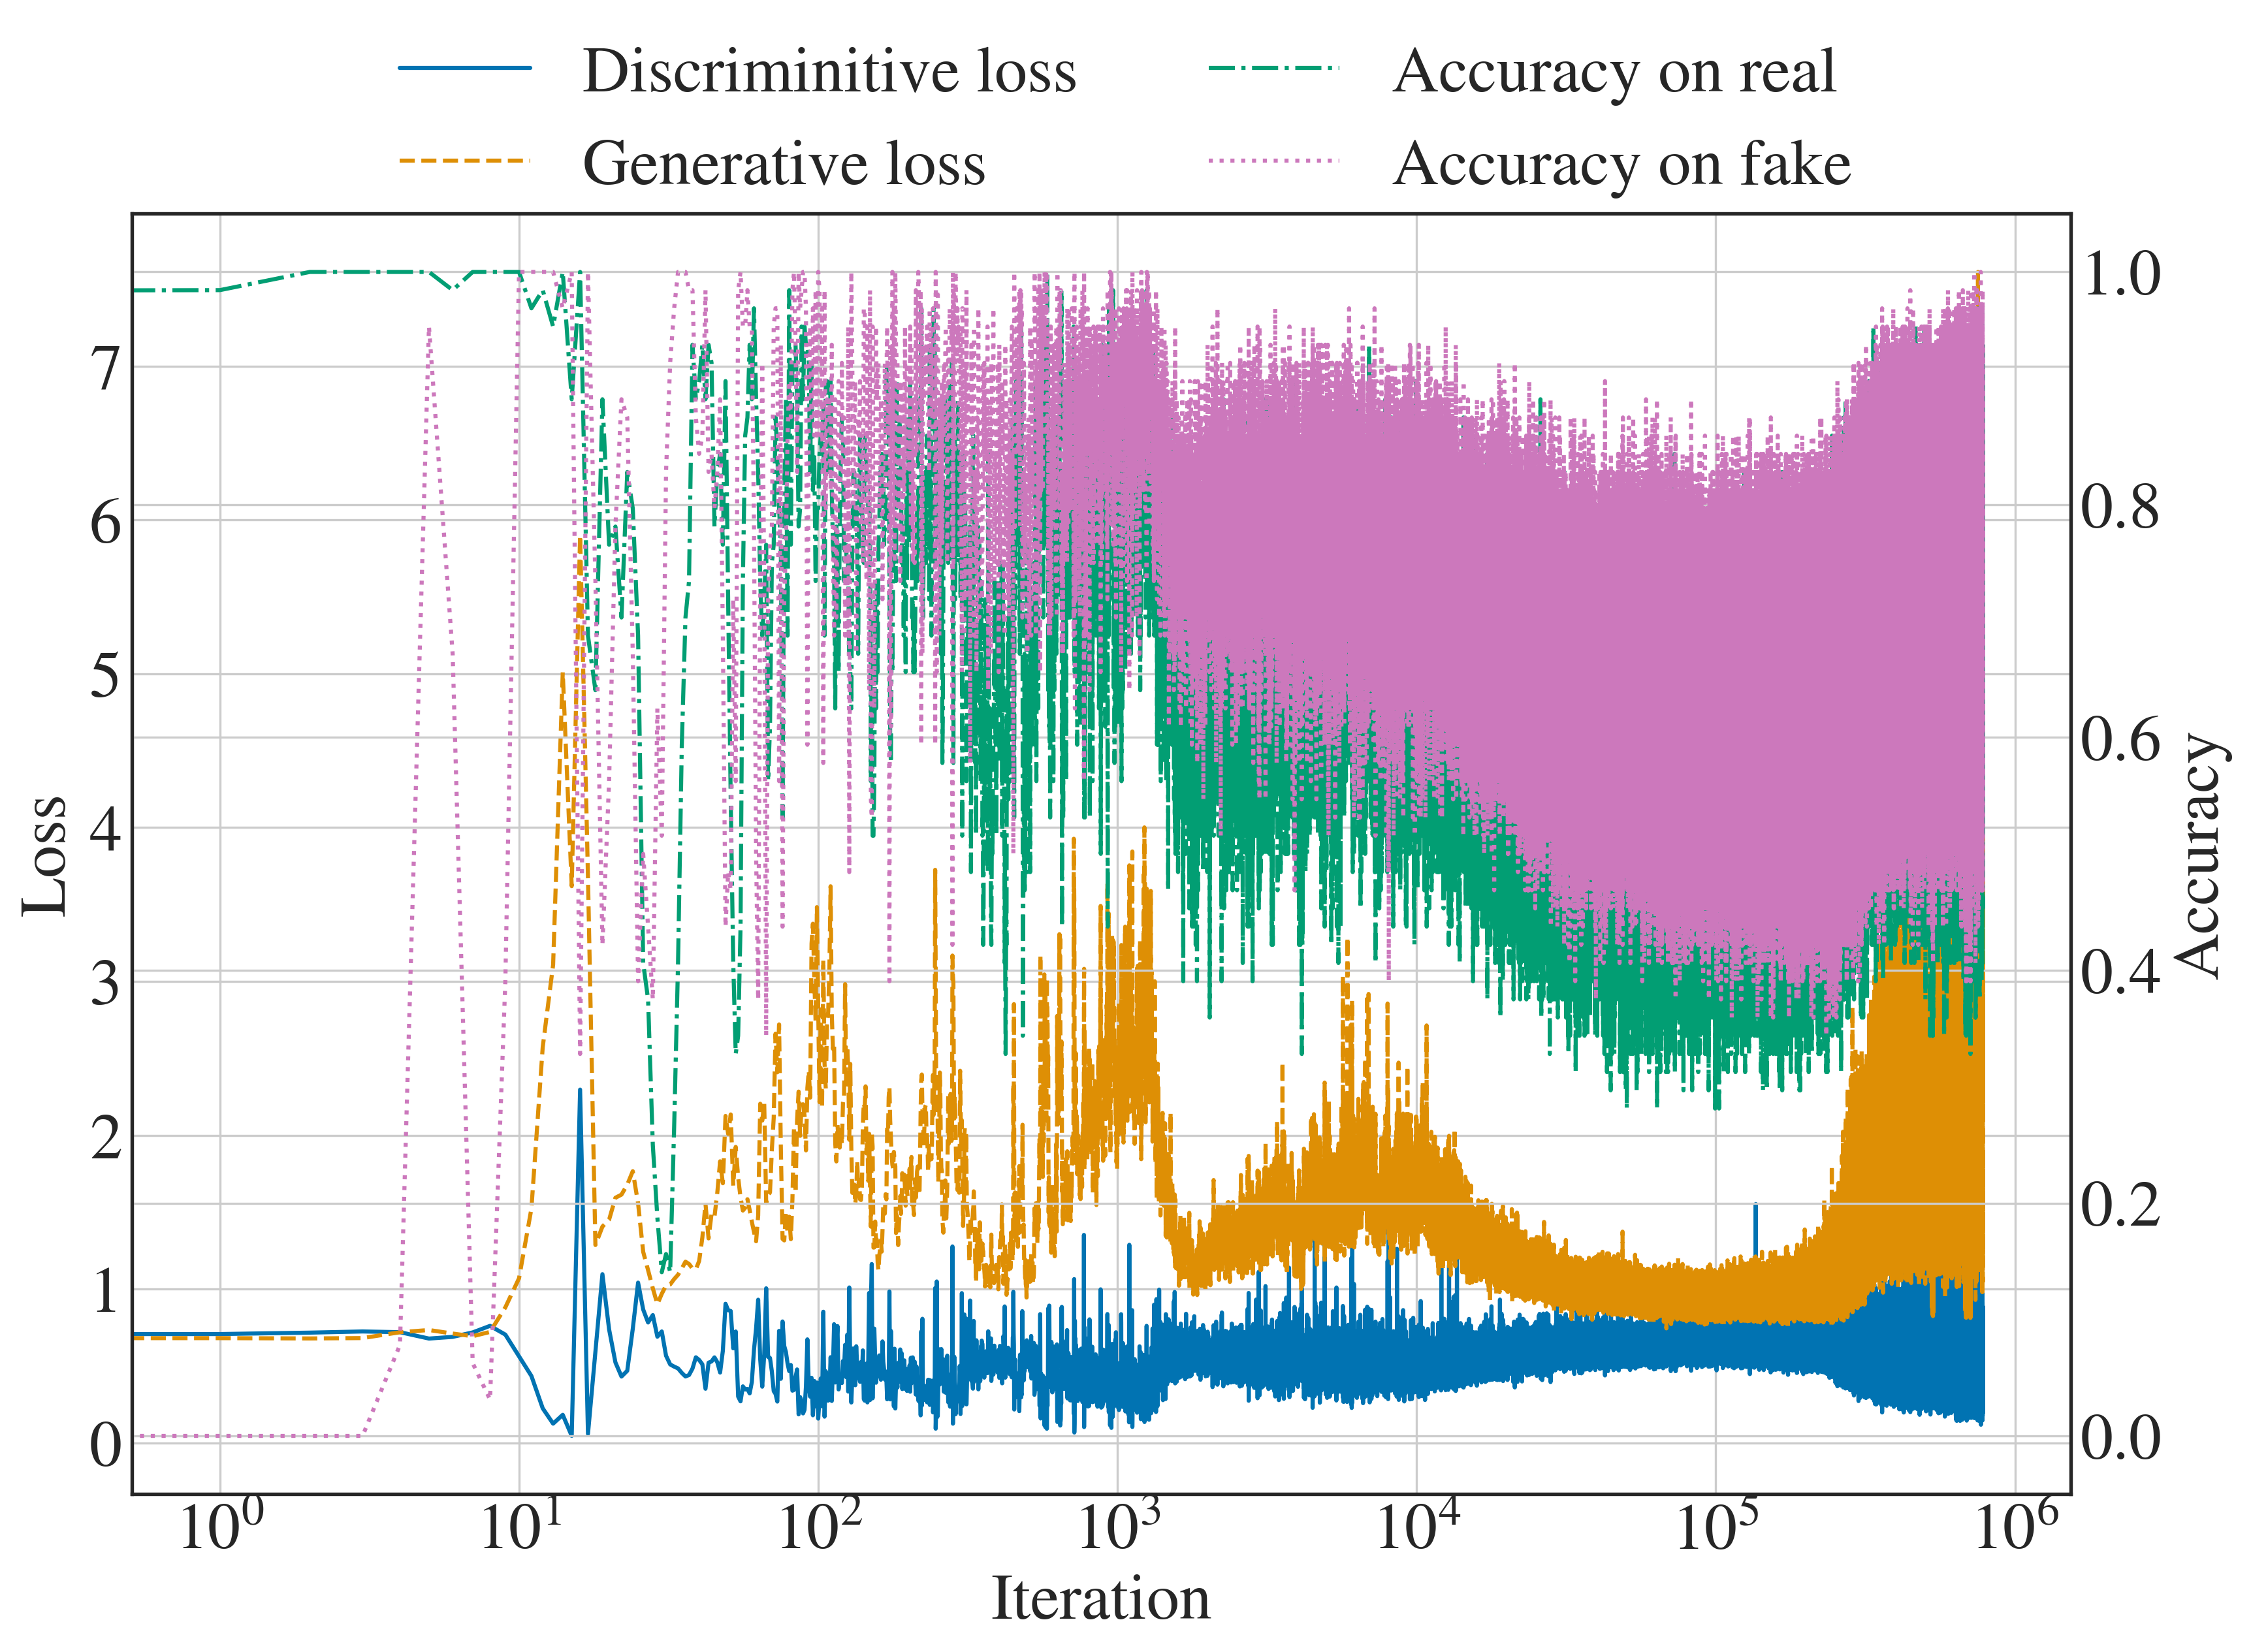
\includegraphics[width=0.85\textwidth]{figures/losses.png}
    \caption{Plot of the discriminator and generator loss and accuracy as a function of epochs. Early in training the losses oscillate as both models attempt to find their equilibrium, after which, both losses vary around a point which signifies stable training. Accuracies on the real and fake data are similar, showing that neither model is stronger than the other.}
    \label{fig:lossplot}
\end{figure}

%%%%%%%%%%%%%%%%%%%%%%%%%%%%%%%%%%%%%%%%%%%%%%%%%%%%%%%%%%%%%%%%%%%%%%%%%%%%%%
\subsection{Conditional GANs}
%%%%%%%%%%%%%%%%%%%%%%%%%%%%%%%%%%%%%%%%%%%%%%%%%%%%%%%%%%%%%%%%%%%%%%%%%%%%%%

% introduce CGANs and ACGANs
%
To gain more control over what a \ac{GAN} is able to generate, a conditional variant
of \acp{GAN} named \acp{CGAN}~\cite{cgan} was introduced by feeding in extra
information into the generator and discriminator such as a class label or
attribute label, $\mathbf{c}$. This simple addition has been shown to work well in practice, for instance in image-to-image translation~\cite{isola2016imagetoimage}. We use one-hot encoding to define the classes, that is, each class resides at the corner points of a \ndimensional{5} cube. For example $\mathbf{c}=[0,1,0,0,0]$ represents the ringdown signal class. The training data and labels are drawn from a joint distribution $p_{\text{data}}(\mathbf{x},\mathbf{c})$, whereas when generating fake data we sample from $\mathbf{c}$ and $p_{\mathbf{z}}(\mathbf{z})$ independently. \cref{equation:GANloss} is modified to include the class labels 
~
\begin{equation}
   \mathop{\text{min}}_{G}  \mathop{\text{max}}_{D} V(D,G) = \mathbb{E}_{\mathbf{x} \sim p_{\text{\text{data}}}(\mathbf{x})} [\text{log} D(\mathbf{x|c})] + \mathbb{E}_{\mathbf{z} \sim p_{\text{z}}(\mathbf{z})} [\text{log}(1-D(G(\mathbf{z|c})))].
 \label{equation:CGANloss}
 \end{equation}
Fig. \ref{fig:gan_comparison} shows the differences in inputs and outputs of a GAN compared with a \ac{CGAN}. We will be using a conditional GAN for this study.

\begin{figure}[h!]
    \begin{subfigure}{.5\textwidth}
     \centering
        %\documentclass{article}
%\usepackage{comment}
%\usepackage{tikz}
%\usetikzlibrary{shapes.geometric, arrows, calc}

%\begin{document}
    
\begin{tikzpicture}[node distance=2cm]

\tikzstyle{zinput} = [rectangle, rounded corners, text centered, draw=black]%, fill=red!30]
\tikzstyle{generator} = [rectangle, rounded corners, text centered, draw=black]%, fill=red!30]
\tikzstyle{X real} = [rectangle, rounded corners, text centered, draw=black]%, fill=red!30]
\tikzstyle{X fake} = [rectangle, rounded corners, text centered, draw=black]%, fill=red!30]
\tikzstyle{X real} = [rectangle, rounded corners, text centered, draw=black]%, fill=red!30]
\tikzstyle{discriminator} = [rectangle, rounded corners, text centered, draw=black]%, fill=red!30]
\tikzstyle{real/fake} = [rectangle, rounded corners, text centered, draw=black]%, fill=red!30]

\tikzstyle{arrow} = [thick,->,>=stealth]

\node (r) [X real] {\textbf{X} real};
\node (f) [X fake, right of = r] {\textbf{X} fake};
\node (G) [generator,above of = f, scale = 2] {\textbf{G}};
\node (z) [zinput] [zinput, above of = G] {\textbf{z} (noise)};
\node (D) [discriminator, below of = f, xshift = -1cm, scale = 2] {\textbf{D}};
\node (rf) [real/fake, below of = D] {real/fake};

\draw [arrow] (z) -- (G);
\draw [arrow] (G) -- (f);
\draw [arrow] (r) edge[out=270,in=90] (D);
\draw [arrow] (f) edge[out=270,in=90] (D);
\draw [arrow] (D) -- (rf);

\end{tikzpicture}
%\end{document}

        \caption{GAN}
    \end{subfigure}
    \begin{subfigure}{.5\textwidth}
     \centering
        \begin{tikzpicture}[node distance=2cm]

\tikzstyle{zinput} = [rectangle, rounded corners, text centered, draw=black]%, fill=red!30]
\tikzstyle{generator} = [rectangle, rounded corners, text centered, draw=black]%, fill=red!30]
\tikzstyle{X real} = [rectangle, rounded corners, text centered, draw=black]%, fill=red!30]
\tikzstyle{X fake} = [rectangle, rounded corners, text centered, draw=black]%, fill=red!30]
\tikzstyle{X real} = [rectangle, rounded corners, text centered, draw=black]%, fill=red!30]
\tikzstyle{discriminator} = [rectangle, rounded corners, text centered, draw=black]%, fill=red!30]
\tikzstyle{real/fake} = [rectangle, rounded corners, text centered, draw=black]%, fill=red!30]
\tikzstyle{coutput} = [rectangle, rounded corners, text centered, draw=black]%, fill=red!30]

\tikzstyle{arrow} = [thick,->,>=stealth]

\node (r) [X real] {\textbf{X} real};
\node (f) [X fake, right of = r, xshift = 0cm] {\textbf{X} fake};
\node (G) [generator,above of = f, scale = 2] {\textbf{G}};
\node (z) [zinput] [zinput, above of = G, xshift = 1cm] {\textbf{z} (noise)};
\node (c) [coutput, left of = z] {\textbf{c} (class)};
\node (D) [discriminator, below of = f, xshift = -1cm, scale = 2] {\textbf{D}};
\node (rf) [real/fake, below of = D] {real/fake};
%\node (co) [coutput, left of = rf, xshift = -0.5cm] {c = 1, 2, ...};

\draw [arrow] (z) edge[out=270,in=90] (G);
\draw [arrow] (c) edge[out=270,in=90] (D);
\draw [arrow] (c) edge[out=270,in=90] (G);
\draw [arrow] (c) edge[out=270,in=90] (r);
\draw [arrow] (G) -- (f);
\draw [arrow] (r) edge[out=270,in=90] (D);
\draw [arrow] (f) edge[out=270,in=90] (D);
\draw [arrow] (D) edge[out=270,in=90] (rf);
%\draw [arrow] (D) edge[out=270,in=90] (co);

\end{tikzpicture}
        \caption{CGAN}
    \end{subfigure}
    \caption{Comparison of the original GAN method and the
conditional-GAN method. $\textbf{G}$ and $\textbf{D}$ denote the generator and discriminator neural networks respectively while $\textbf{X}~\text{real}$ and $\textbf{X}~\text{fake}$ represent samples drawn from the training set and the generated set. For CGANs the training data requires a label denoting
its class that is also fed to the generator which then learns to generate
waveforms based on the input label.}
\begin{comment}
~\chris{Overall it's a bit basic and doesn't indicate either the
2 competing training steps or any aspect of the loss or specify that $x$ and
$z$ (and $c$) are drawn from distributions already defined in the text. Maybe it's OK without
that. As for the CGAN, I'm troubled by the fact that there is only one $c$ box.
It implies that the same $c$ value is given to each real and fake $x$ data when
in fact each $x$ sample has it's own randomly drawn $c$ value.}
\end{comment}
\label{fig:gan_comparison}
\end{figure}

%%%%%%%%%%%%%%%%%%%%%%%%%%%%%%%%%%%%%%%%%%%%%%%%%%%%%%%%%%%%%%%%%%%%%%%%%%%%%%
%%%%%%%%%%%%%%%%%%%%%%%%%%%%%%%%%%%%%%%%%%%%%%%%%%%%%%%%%%%%%%%%%%%%%%%%%%%%%%
\section{Training data and architecture} \label{Method}
%%%%%%%%%%%%%%%%%%%%%%%%%%%%%%%%%%%%%%%%%%%%%%%%%%%%%%%%%%%%%%%%%%%%%%%%%%%%%%
%%%%%%%%%%%%%%%%%%%%%%%%%%%%%%%%%%%%%%%%%%%%%%%%%%%%%%%%%%%%%%%%%%%%%%%%%%%%%%

\begin{comment}
\begin{itemize}
\item Need to introduce the scheme you propose to use
\item A paragraph or subsection on the data generation being very clear on all
5 waveform models and the prior parameter space for each \ding{51}
\item A subsection on the design of the network architecture \ding{51}
\item A subsection on the "box" and why we implement it \ding{51}
\item A subsection on the training of the network - give rough timings and rule
of thumb decisions made
\item Do not discuss the results here 
\end{itemize}
\end{comment}

% introduce the training data
%
\begin{figure}
    \centering
    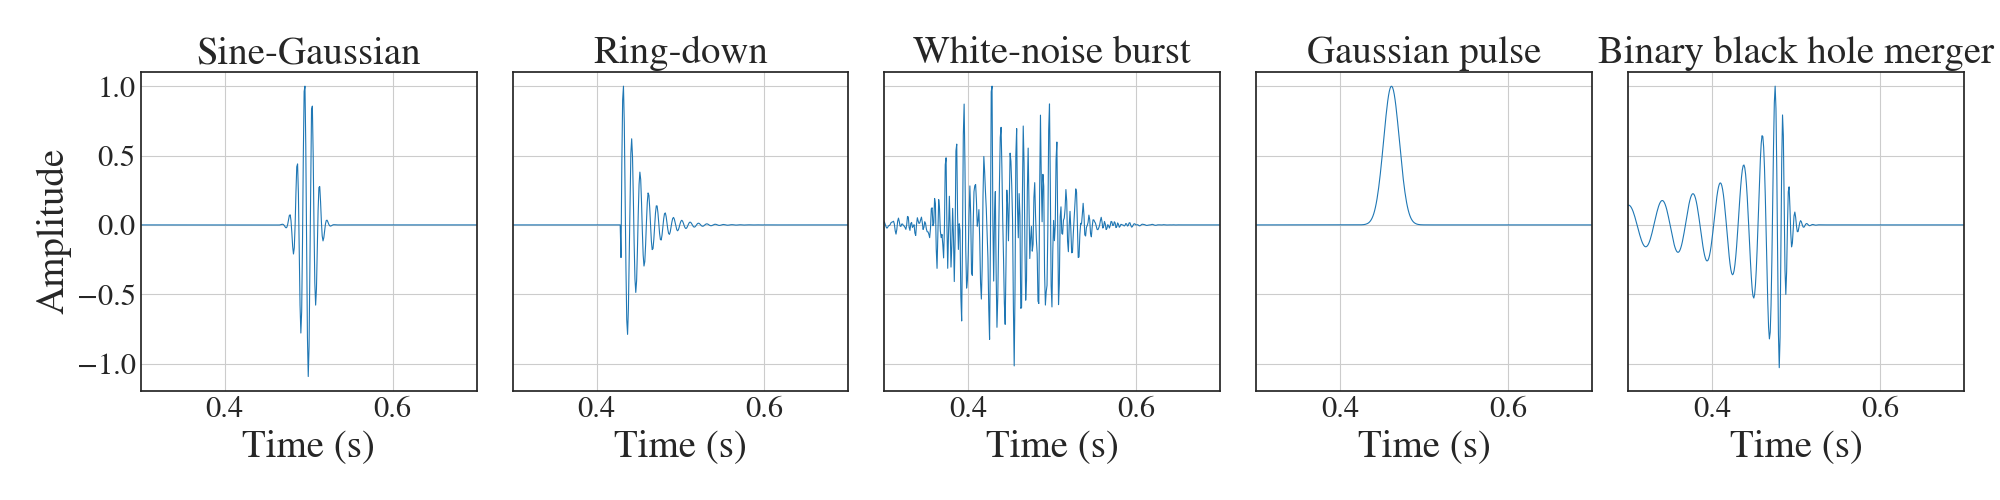
\includegraphics[width=\textwidth]{figures/training-sample.png}
    \caption{Examples of the five different waveforms that were used in training the \ac{GAN} for this study. Values of the parameters were selected randomly from uniform distributions from \cref{Tab:training_parms}. \michael{Ringdown is hyphenated here, this is the only place}}
    \label{fig:training_waveforms}
\end{figure}
% introduce the signal models
%
We propose a signal generation scheme using a \ac{CGAN} trained on burst-like waveforms. We call this \texttt{McGANn}\footnote{https://github.com/jmcginn/McGANn} and it is a \ac{CGAN} trained on five signal classes each spanning a range of prior signal parameters. The signal classes are:

% list the 5 waveform classes
%
\begin{itemize}
%
\item {\bf Sine-Gaussian}: $h_{\text{sg}}(t) = A \exp\left[ - (t-t_{0})^2 /
\tau^2 \right] \sin (2 \pi f_0 (t-t_0) + \phi)$, \michael{Could capitalise SG here?} a sinusoidal wave with a Gaussian
envelope characterised by a central frequency, $f_0$, amplitude, $A$, time of arrival, $t_{0}$ and phase, $\phi$ which is uniformly sampled between $[0, 2\pi]$ \michael{The commas here are a bit of mess, I find it hard to read I think either remove the comma before each symbol or use brackets? The same applies to this whole list. I've removed them in the next point, see what you think.}. 
%
\item {\bf Ringdown}: $h_{\text{rd}}(t) = A \exp \left[-{(t-t_0)} / {\tau}
\right] \sin(2 \pi f_0 (t-t_0) + \phi)$, with frequency $f_0$ and duration $\tau$, amplitude $A$, time of arrival $t_{0}$ and phase $\phi$ which is uniformly sampled between $[0, 2\pi]$. 
%
\item {\bf White noise bursts}: $h_{\text{wn}}(t_j) = Ag_j\exp\left[ -
(t-t_{0})^2 / \tau^2 \right]$ where $g_j$ are drawn from a zero mean unit
variance Gaussian distribution with a Gaussian envelope of duration $tau$.
%
\item {\bf Gaussian pulse}: $h_{\text{gp}}(t) = \exp(-t^2 / \tau^2)$ with
duration parameter $\tau$.
%
\item {\bf Binary black hole}: Simulated using the IMRPhenomD
waveform~\cite{Khan_2016} routine from LALSuite~\cite{lalsuite} which models
the inspiral, merger and ringdown of a \ac{BBH} waveform. The component masses
lie in the range of [30,70] $\textrm{M}_{\odot}$ with zero spins and we fix
$m_1>m_2$. The mass distribution is approximated by a power law with
index of 1.6~\cite{Abbott_2019}. The inclinations are drawn
such that the cosine of the angles lies uniformly in the range [-1,1] and we only use the plus polarisation.
%
\end{itemize}
%
The location of the peak amplitude of the waveforms (corresponding to the
mid-points of all but the ringdown and \ac{BBH} classes) are randomly drawn from a uniform distribution to
be within $[0.4, 0.6]$ seconds from the start of the 1 sec time interval and all
training waveforms are sampled at 1024 Hz.  The parameter prior ranges are
defined in~\cref{Tab:training_parms} and a sample of training waveforms are shown in \cref{fig:training_waveforms}. All training data is rescaled such that their amplitudes peak at 1.

\begin{table}[!h]
\centering
\caption{The parameters used in generating the training data. Each parameter is drawn uniformly in the below ranges. \michael{You've used a mix of - and N/A, are they the same thing or do they indicate something different?} \jordan{I changed N/A to "-" as they do really mean the same thing.}}
%\footnotesize
\begin{tabular}{@{} l l l l l l }
\br
\hline
 Waveform & Central frequency  & Decay & Central time epoch & Mass range \\
 & (Hz) & (s) & (s) & ($\textrm{M}_{\odot}$) \\
\mr
Sine-Gaussian & 70 - 250 & 0.004 - 0.03 & 0.4 - 0.6 & -  \\  
Ringdown & 70 - 250 & 0.004 - 0.03 & 0.4 - 0.6 & - \\
white noise burst & 70 - 250 & 0.004 - 0.03 & 0.4 - 0.6 & -  \\
Gaussian pulse & - & 0.004 - 0.03 & 0.4 - 0.6 & -  \\
BBH & - & - & - & 30 - 70  \\
 \br
\end{tabular}\\
\label{Tab:training_parms}
\end{table}
\normalsize

%%%%%%%%%%%%%%%%%%%%%%%%%%%%%%%%%%%%%%%%%%%%%%%%%%%%%%%%%%%%%%%%%%%%%%%%%%%%%%
\subsection{Architecture details}
%%%%%%%%%%%%%%%%%%%%%%%%%%%%%%%%%%%%%%%%%%%%%%%%%%%%%%%%%%%%%%%%%%%%%%%%%%%%%%
%
% Introduce some architecture features
%
% describe the hyperparameter tunings
%
Neural networks and subsequently \acp{GAN} have multiple parameters a developer
can tune when designing the model and these are referred to as hyperparameters.
The final network design used in this work comes was developed through trial and
error and the initial designs influenced by the available literature. We found
that the \ac{GAN} performed better with both networks having the same number of
layers and neurons which encourages even
competition between the generator and discriminator.  After tuning the multiple
hyperparameters (see \cref{Tab:gan_training_parms}), the \ac{GAN} was trained on
$10^5$ signals  drawn from a categorical
distribution with equal propabilities for each class of
sine-Gaussian,
ringdown, white noise bursts, Gaussian pulse and \acp{BBH}.

The design of the networks is influenced by \cite{Radford2015} in which they use a \ac{DCGAN} architecture. The generator model is fully convolutional, upsampled using strided transposed convolutions with batch normalisation in the first layer and ReLU activations throughout with the exception of a linear activation for the output layer. The use of a linear activation guarantees the output can have negative and positive outputs. Each transposed convolutional layer uses a kernel size of 18 and stride of 2. The discriminator network mirrors that of the generator without batch normalization, using LeakyReLU activations, SpatialDropout, and a 2-stride convolution for downsampling. The discriminator output is a single node with sigmoid activation that can be interpreted as a probability of the the signal being real and both models are trained with binary cross entropy \cref{eqn:crossentropy}. The full architecture description can be seen in~\cref{Tab:gan_training_parms}.

All models were designed with the Python Keras library \cite{} and TensorFlow \cite{} \michael{Just a reminder these are missing} and trained on a GeForce RTX 2080 Ti GPU. We train the networks for 500 epochs which takes $\mathcal{O}(10)$ hours and save the model at each epoch. We choose an appropriate model by visually inspecting the generations at a point of convergence on the loss plot. 
%%%%%%%%%%%%%%%%%%%%%%%%%%%%%%%%%%%%%%%%%%%%%%%%%%%%%%%%%%%%%%%%%%%%%%%%%%%%%%
\section{Results} \label{results}
%%%%%%%%%%%%%%%%%%%%%%%%%%%%%%%%%%%%%%%%%%%%%%%%%%%%%%%%%%%%%%%%%%%%%%%%%%%%%%


\begin{comment}
\begin{itemize}
\item Begin by outlining the type of results you will be presenting
\item A subsection on the general quality of generated waveforms - we may need
to have overlaps between generated wavefoms and training data (maybe)
\item A subsection on the descriminator - maybe a confusion matrix?
\item a subsection on the latent space varaition within each class - fixed
class, sliding in latent space.
\item A subsection on the class space variation - fixed latent space and
sliding in the class space.
\item A final subsection on the general waveform model based on random latent
and class space locations.
\item Make no conclusions.
\end{itemize}
\end{comment}

% describe the main idea
%
Given a \ndimensional{100} vector drawn from a normal distributed latent space and a one-hot encoded class
label, the GAN is able to generate burst-like waveforms generalised from the
training set. We set out by describing the quality of generated waveforms and
how they compare to the training set. We then explore the structure of the
latent and class spaces by interpolating between points in these spaces. We
test three methods of sampling from the class space that can be used to generate new signals composed of weighted elements of each training class.

\begin{figure}[!h]
    \centering
    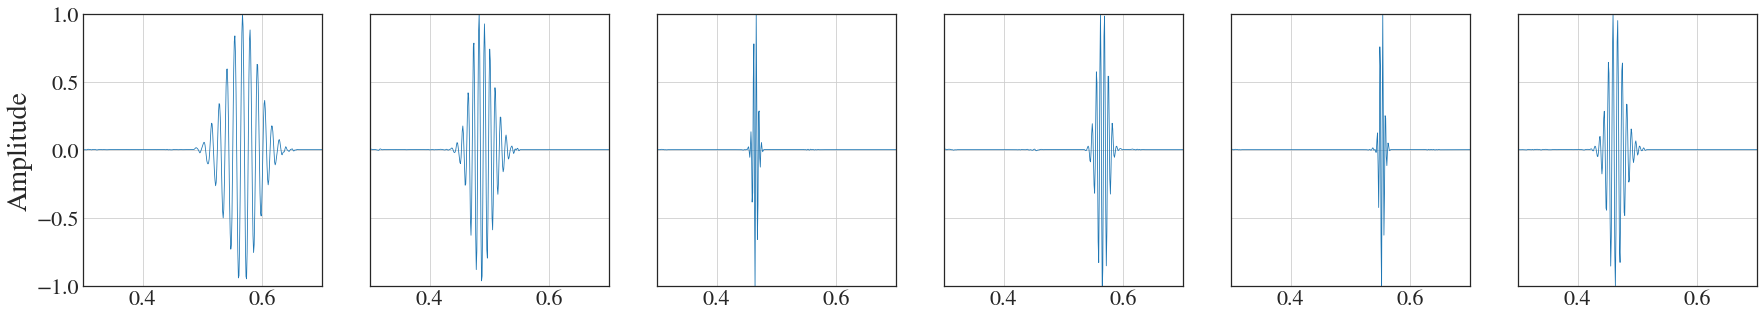
\includegraphics[width=\textwidth]{figures/generations/sg.png}
    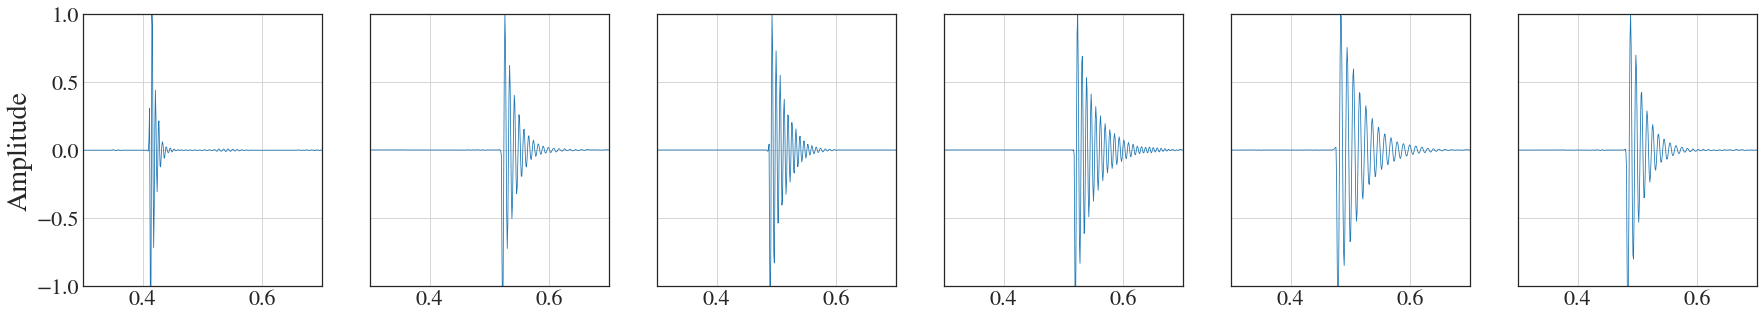
\includegraphics[width=\textwidth]{figures/generations/rd.png}
    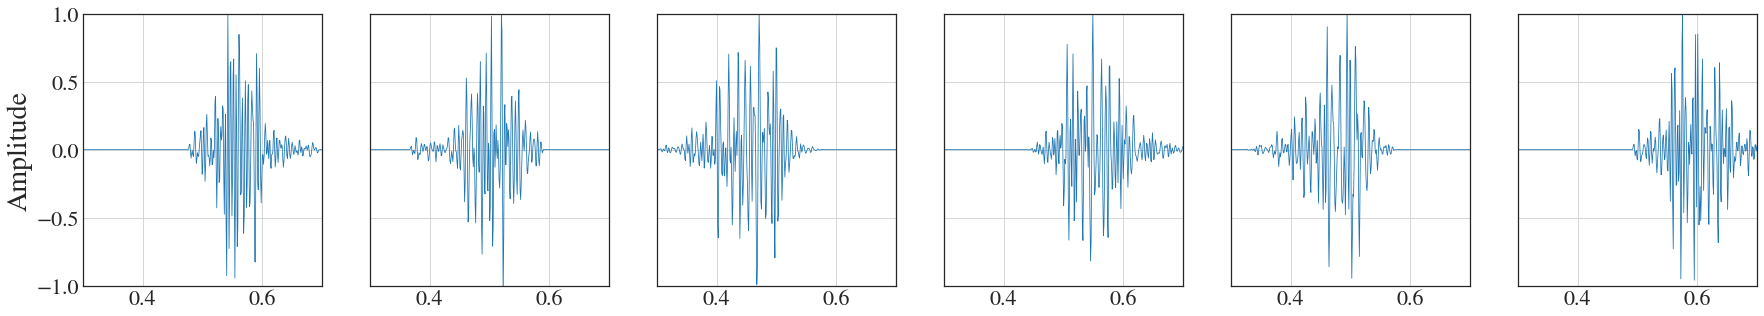
\includegraphics[width=\textwidth]{figures/generations/wnb.png}
    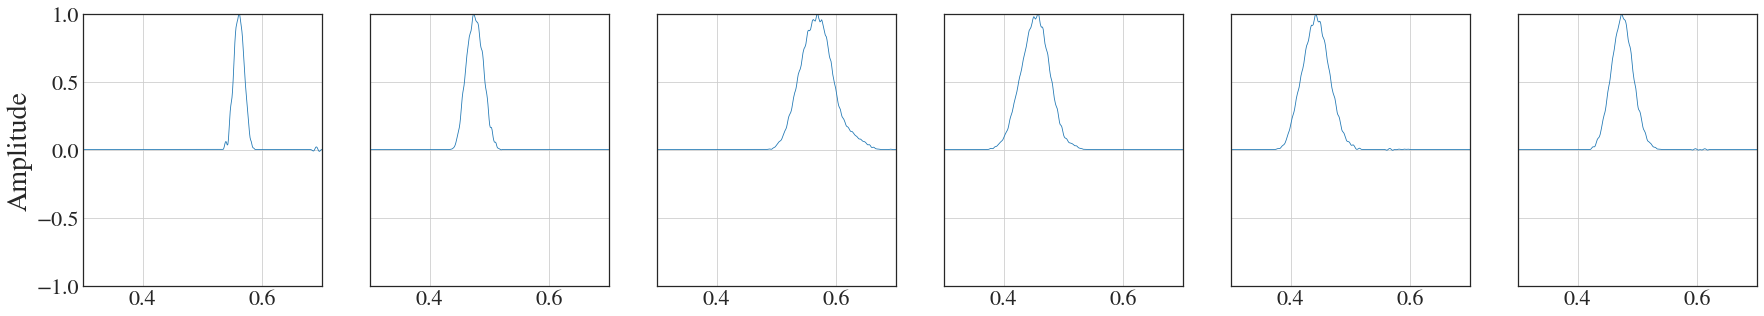
\includegraphics[width=\textwidth]{figures/generations/blip.png}
    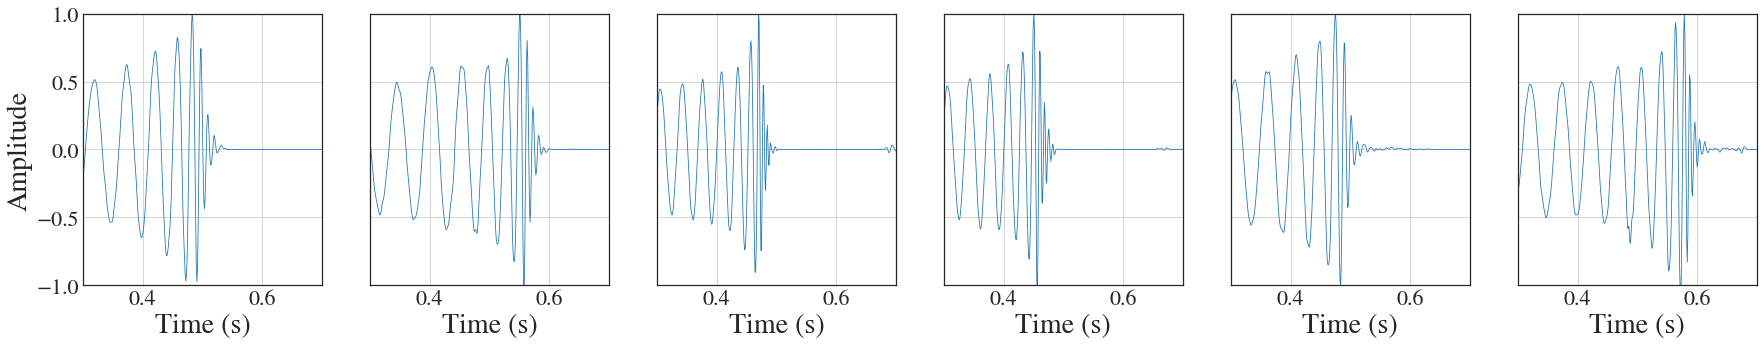
\includegraphics[width=\textwidth]{figures/generations/bbh.png}
    \caption{\ac{GAN} Generated waveforms plotted as a function of time. The latent space inputs for each panel are randomised and each row is assigned one of the five class vectors. By row: sine-Gaussian, ringdown,
white noise burst, Gaussian pulse, binary black hole merger. For ease of viewing, the $x$-axis for all panels spans the mid 50\% of the output range. \michael{I think we mentioned increasing the y-axis limits a little so it's clearer the signals end at $\pm 1$}}
\label{fig:gen_signals} 
\end{figure}
%%%%%%%%%%%%%%%%%%%%%%%%%%%%%%%%%%%%%%%%%%%%%%%%%%%%%%%%%%%%%%%%%%%%%%%%%%%%%%
\subsection{Known class signal generation}
In \cref{fig:gen_signals} we show conditional signal generations using our generator network. We can see the generations are of very good quality \michael{Personally don't like using good quality without a metric to quantify things.} and appear as though they could have plausibly come from the training set. We can also see that the model has learned the overall characteristics of the five training classes and is able to disentangle each class and associate them with the conditional input. Additionally, as the latent variable changes we see indirect evidence of variation within the parameter space for a given class. For instance \cref{fig:gen_signals} shows how signals vary in frequency, central epoch, decay timescale, and phase. The \acp{GAN} ability to generate a variety of signals for various latent space input indicates stable training and no mode collapse. 
\begin{figure}[!h]
    \centering
    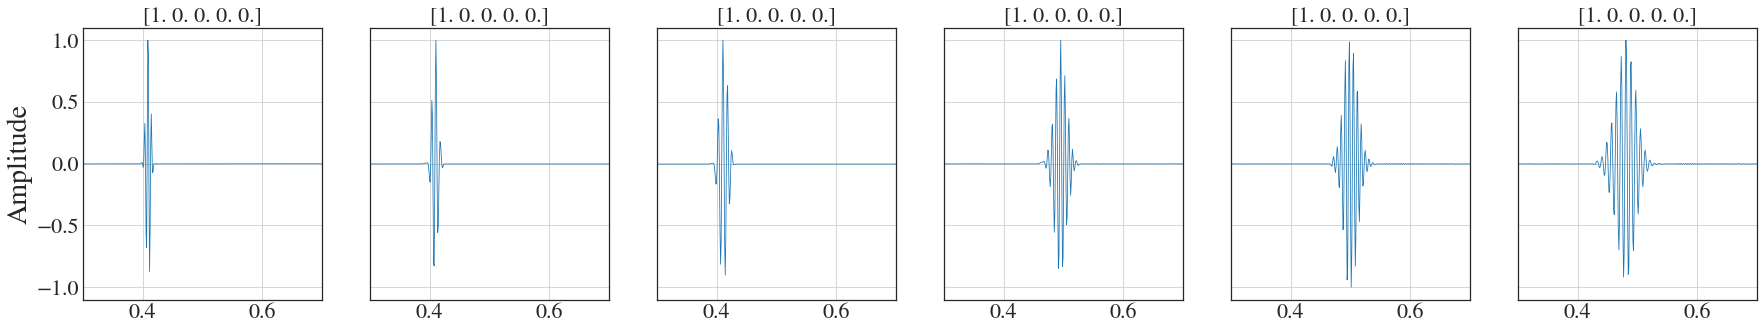
\includegraphics[width=\textwidth]{figures/generations/z_interp_sg.png}
    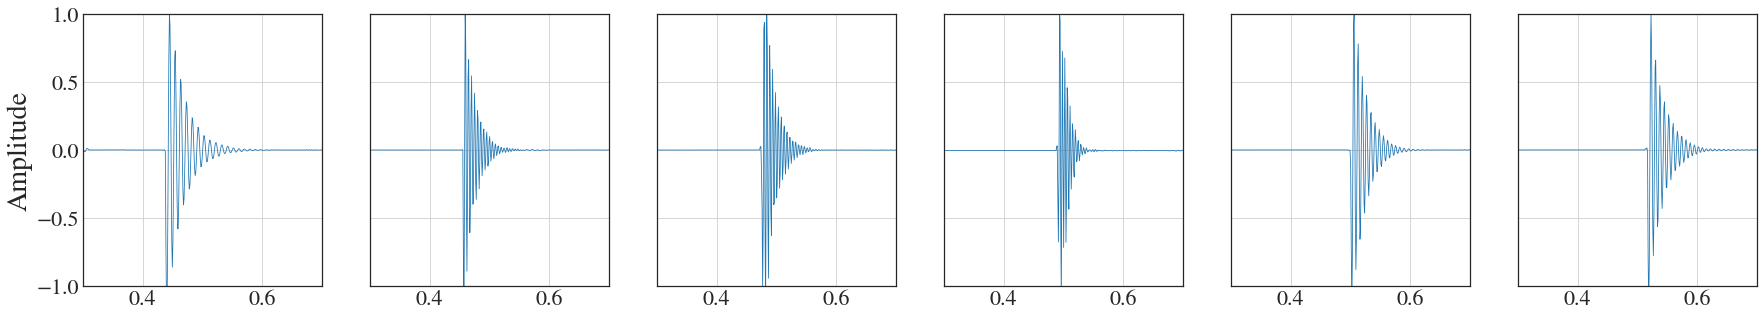
\includegraphics[width=\textwidth]{figures/generations/z_interp_rd.png}
    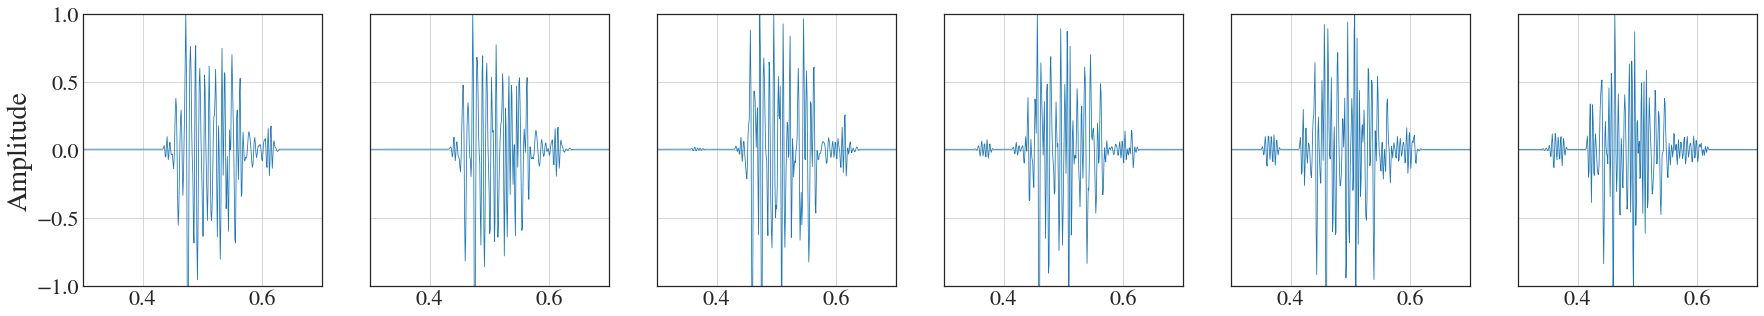
\includegraphics[width=\textwidth]{figures/generations/z_interp_wnb.png}
    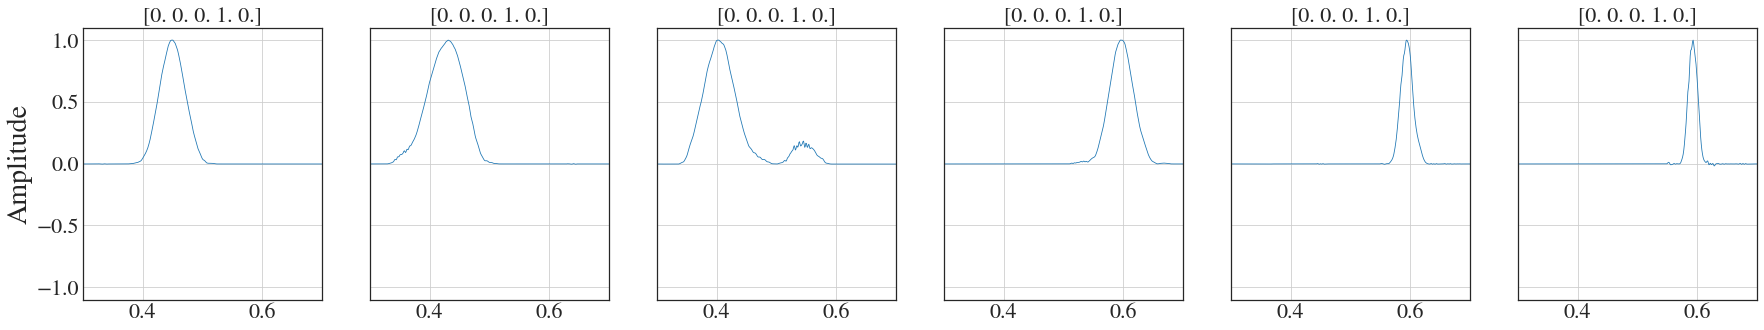
\includegraphics[width=\textwidth]{figures/generations/z_interp_blip.png}
    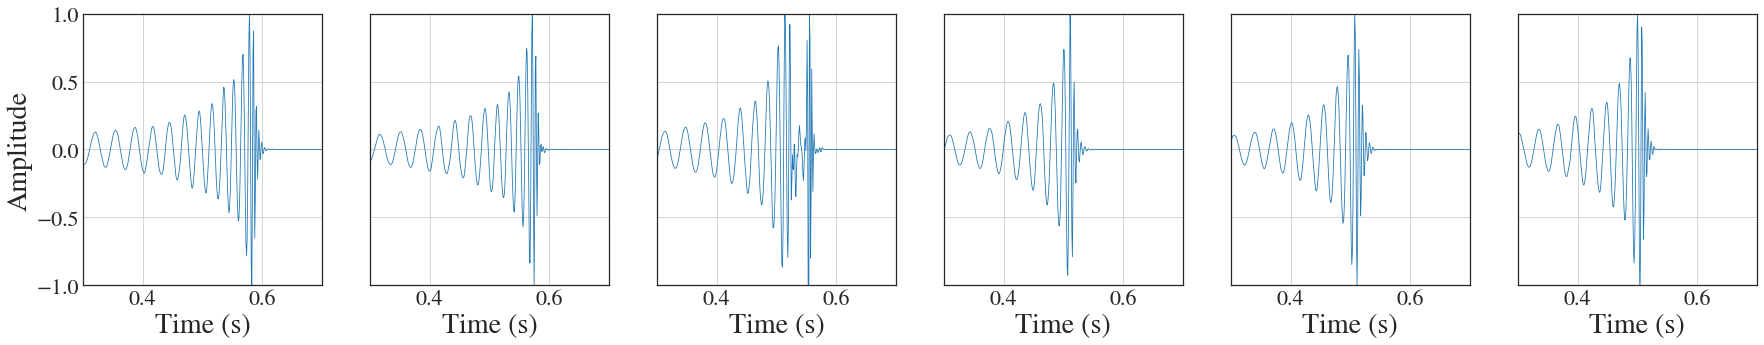
\includegraphics[width=\textwidth]{figures/generations/z_interp_bbh.png}
    \caption{\ac{GAN} generated interpolated waveforms plotted as a function of time showing latent space interpolations. For each interpolation two different points were randomly chosen in the latent space and represent the first last panels in each row. The panels between represent signals generated using linearly interpolated vectors between these two points. Each row keeps its class vector constant throughout the latent space interpolation. By row: sine-Gaussian, ringdown, white noise burst, Gaussian pulse, binary black hole merger. For ease of viewing, the $x$-axis for all panels spans the mid 50\% of the output range.}
    \label{fig:z_interp}
\end{figure}
%%%%%%%%%%%%%%%%%%%%%%%%%%%%%%%%%%%%%%%%%%%%%%%%%%%%%%%%%%%%%%%%%%%%%%%%%%%%%%
\subsection{Interpolation within the latent space}
%
% explain what we are planning to show here
%
 We have shown that the generator produces quality signals and that the model responds well to randomly sampled Gaussian latent vectors. We now assume that during training the generator has learned a mapping from a Gaussian latent space to signal space and that this mapping is a smooth function of the underlying latent space. To verify this, we fix the class vector input and linearly interpolate between two randomly chosen points in the latent space (different for each class). In \cref{fig:z_interp} we show the generated waveforms, with the class vectors held constant along each row. We can see that each plot shows plausible waveforms suggesting that the generator has constructed a smooth traversable, space. We note that the relationship between the latent space location and the physical signal parameters is intractable, and hence the initial and final latent space locations (moving left to right in \cref{fig:z_interp}) simply represent random possible signals learned from the training set prior. During training the network should have learned how to smoothly represent the underlying features of a signal as a function of latent space location. For example, the linearly interpolated transition through the latent space for the Gaussian pulse signal shows a shift to earlier epoch and larger decay timescale. In contrast, the transition for the ringdown signal appears to pass through a localised region of latent space consistent with higher central frequency. 
%%%%%%%%%%%%%%%%%%%%%%%%%%%%%%%%%%%%%%%%%%%%%%%%%%%%%%%%%%%%%%%%%%%%%%%%%%%%%%
\subsubsection{Interpolation between pairs of classes}

While the \ac{GAN} is trained on distinct one-hot encoded classes, we may test arbitrary points in the \ndimensional{5} class space to produce indistinct or hybrid waveforms. In order to explore the class space, in \cref{fig:c_interp} we show results where the latent vector is held constant but we instead linearly
interpolate within the one-hot encoded class space between pairs of the well-defined training class locations. In this scenario we highlight that the \ac{GAN} has not yet probed this intermediate class space during its training and therefore we are reliant on the generator having learned any underlying class space relationships between the 5 training classes. The results show that for each case that the generated signals show distinct characteristics of the respective class pairs at most stages of the transition. We note that transitions in some cases appear to be rather abrupt, e.g., between the Gaussian pulse and the \ac{BBH}, \chris{but we point out that this feature, whilst not uncommon, is a strong function of the random latent space location.} \michael{We sometimes hyphenate class space and sometimes don't}
%
\begin{figure}[!h]
    \centering
    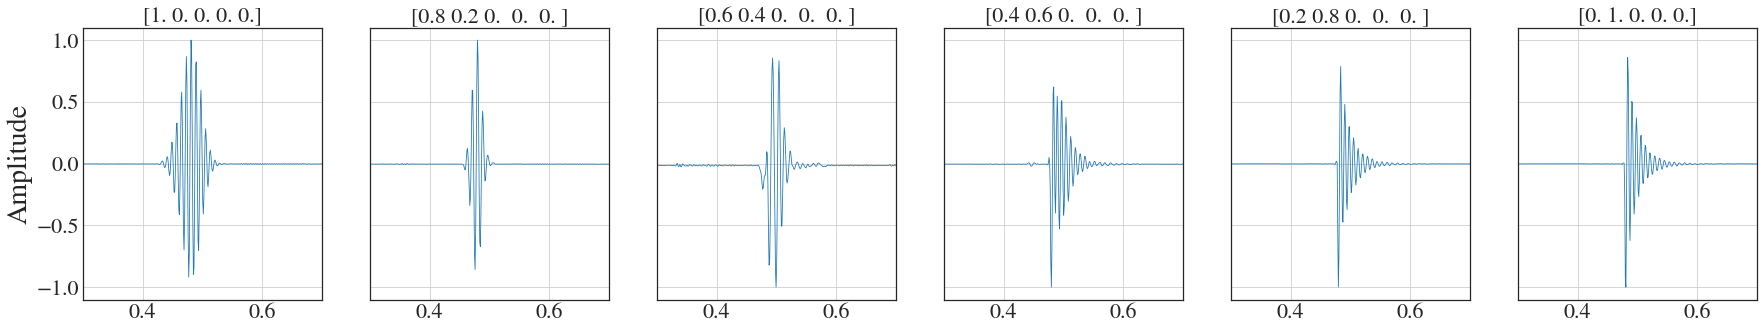
\includegraphics[width=\textwidth]{figures/generations/sg-rd.png}
    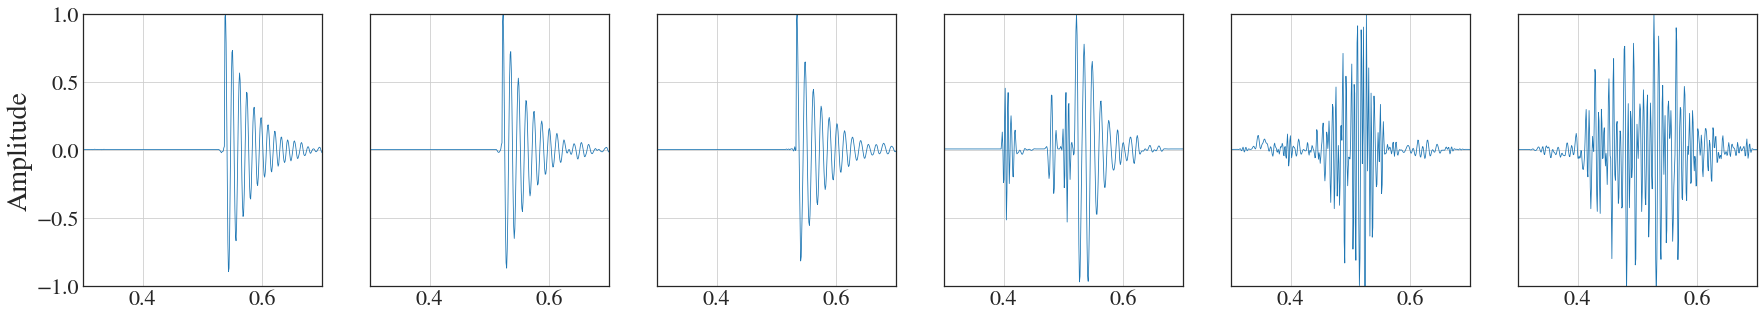
\includegraphics[width=\textwidth]{figures/generations/rd-wnb.png}
    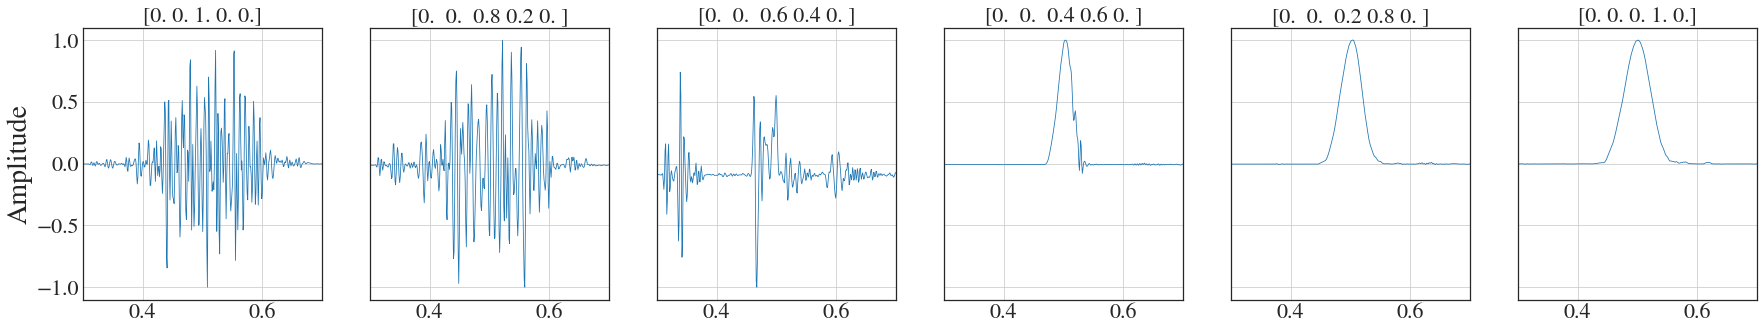
\includegraphics[width=\textwidth]{figures/generations/wnb-blip.png}
    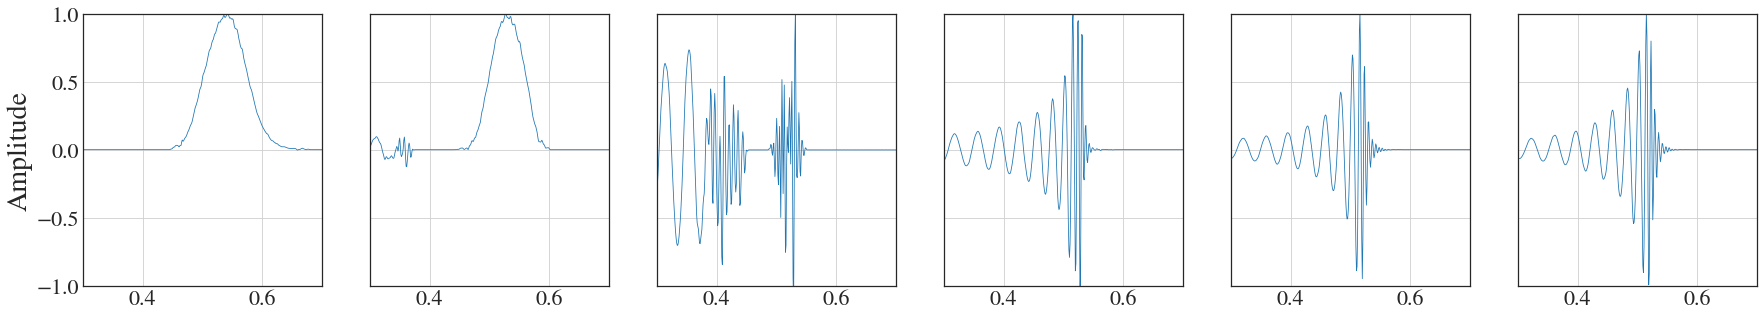
\includegraphics[width=\textwidth]{figures/generations/blip-bbh.png}
    \caption{\ac{GAN} generated class interpolated waveforms as a function of time showing class space interpolations. A single latent space vector is used for all generations and is chosen randomly in the latent space. Each row shows generations using linearly interpolated classes as inputs to the generator. By row top to bottom: Sine-Gaussian to ringdown, ringdown to white noise burst, Gaussian pulse to BBH.\chris{add class vectors on each panel}}
    \label{fig:c_interp}
\end{figure}
%
\subsection{General points within the class space}
We have shown that the \acp{GAN} latent space and class space \michael{Same comment about hyphenation for latent space.} have structure that can be navigated via interpolation between pairs of locations within each respective space. Taking a step further, we can sample from the class space in novel ways to create new inputs for the generator. These new points are categorised by the method used to sample from the class space. The methods we use are divided into the following: 
%
\begin{itemize}
%
\item {\bf Vertex}: Points that lie at the corners of the \ndimensional{5} class space. These class space locations are equivalent to the training set locations and are our closest generated representation of the training set.
%
\item {\bf Simplex}: This class vector we define as uniformly sampled points on a simplex, which is a generalization of a triangle in $k$-dimensions. We sample uniformly on the $k=4$ simplex that is embedded in the \ndimensional{5} class hyper-cube. In practice we use the equivalent of sampling points from a $k=4$ Dirichlet distribution. It is useful to think of the simplex as the hyper-plane that intersects all 5 training classes. It is a subspace of the Uniform method.  
%
\item {\bf Uniform}: Each of the entries in the class vector is sampled from a uniform distribution $\text{U}[0,1]$. This is equivalent to sampling uniformly within the \ndimensional{5} one-hot encoding hyper-cube.
%
\end{itemize}

The vertex points are the most straightforward where one element of the class vector contains one and the other elements are zero. these points are equivalent to the class vectors that the \ac{GAN} is trained on e.g., $\mathbf{c} = [1,0,0,0,0]$ would correspond to a sine-Gaussian generation. Uniform class vectors with each element sampled from a uniform distribution are equivalent to a random draw from a \ndimensional{5} hyper-cube. Uniformly sampling generates class space locations up to a maximum distance of unity from the closest class e.g. $[0,0,0,0,0]$ is of distance 1 away from all classes (as is $[1,1,1,1,1]$ \michael{Isn't this point further? $\sqrt{(1-1)^2 + 1^2 + 1^2 + 1^2 + 1^2} = \sqrt{4} = 2$?}). For simplex class vectors, we sample from the simplest hyper-surface that intersects all the classes and has a symmetry such that no training class location (any vertex) is favoured over any other. For our \ndimensional{5} case this corresponds to a 4-simplex manifold. Sampling from the simplex can be seen as sampling from the simplest space that spans between the training classes.   

In \cref{fig:simplexd_samples} we show generations conditioned on class vectors drawn randomly from the 4-simplex. There are large variations in the signals with some having characteristics strongly resembling the training classes, although this can be partially explained through the random draws from the simplex as there is finite probability that one class entry will dominate over the others (i.e., the class space location is close to a vertex). For instance the generations that look more like sine-Gaussians than hybrid waveforms generally have a larger value placed in the first class space element than others. Similarly \cref{fig:uniform_samples} shows generations conditioned on class vectors drawn uniformly in the unit hyper-cube. These types of generations tend to exhibit more noise and some tend to be generated with very low amplitude prior to being re-scaled to have maximum amplitude of unity. Both methods of generating hybrid waveforms, however, do produce signals that appear to share characteristics from the training set but still be distinct in signal morphology. Upon inspection of a larger collection of waveform generations from both methods we do see a tendency for the uniform hyper-cube approach to generate a wider variety of hybrid waveforms that are more visually distinct from the training set. This is to be expected given that the simplex class space is a subset of the hyper-cube and does not explore regions of the class space as far from the training set vertices.

\begin{comment}
~\chris{Also, discuss the corresponding figure! There has to be comment on the
features of simplex vs box generations as well as general comments about how
the GAN likes to mix signals up. Pick on specific examples and comment on
interesting or annoying features.We can expect a priori that the uniformly sampled space (which contains the simplex as a subspace) will allow for some level of extrapolation.}

\michael{You could also point to \cref{fig:gen_signals} since you have figures for Uniform and Simplex}

~\chris{I have an idea for the plots. Could we have a colour coding system
where each class gets a colour and then when you mix them you plot it with the
mixed colours - you average the RGB values. Maybe everything would look brown?
Worth a try?}
\end{comment}

\begin{figure}
    \centering
    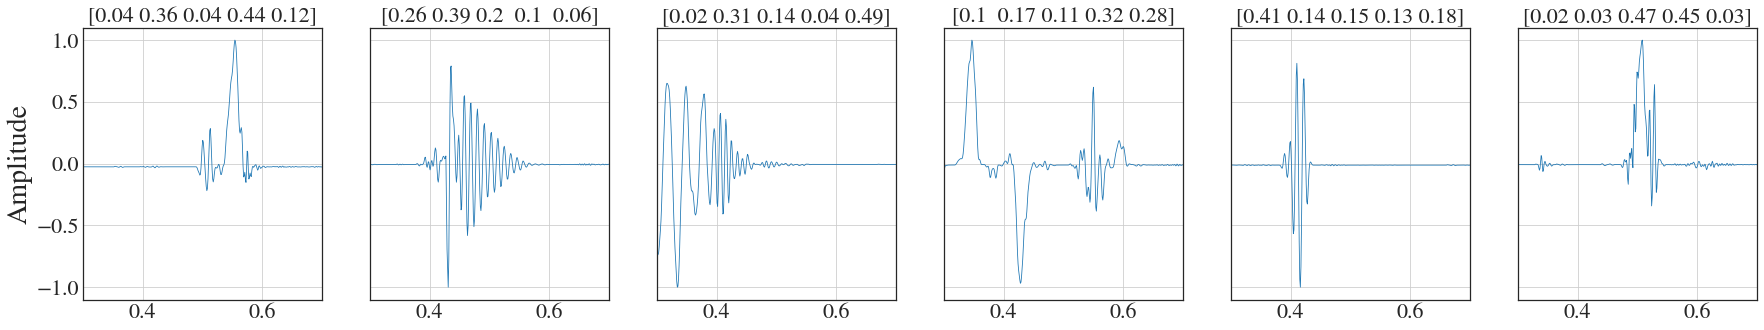
\includegraphics[width=\textwidth]{figures/generations/simplex_sample1.png}
    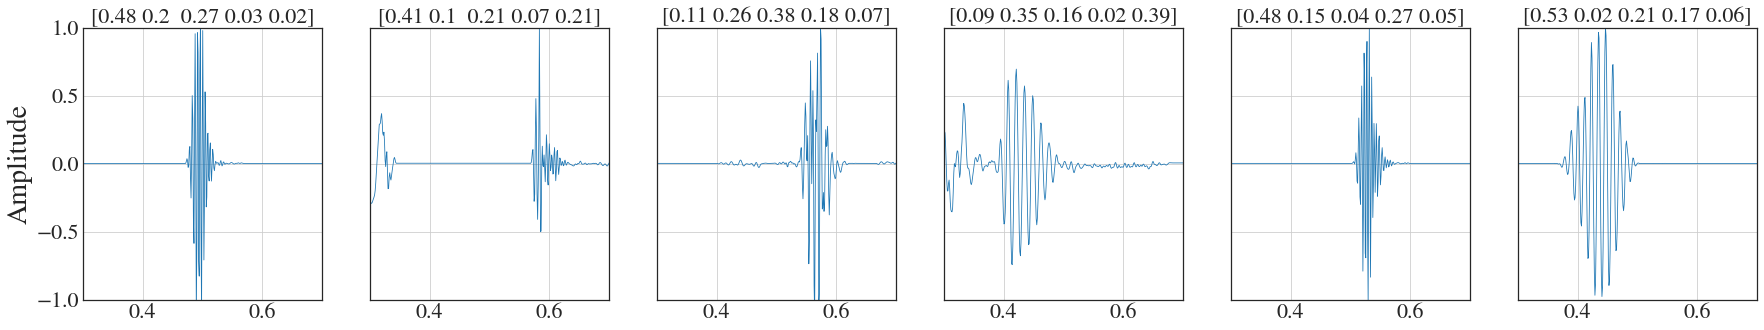
\includegraphics[width=\textwidth]{figures/generations/simplex_sample2.png}
    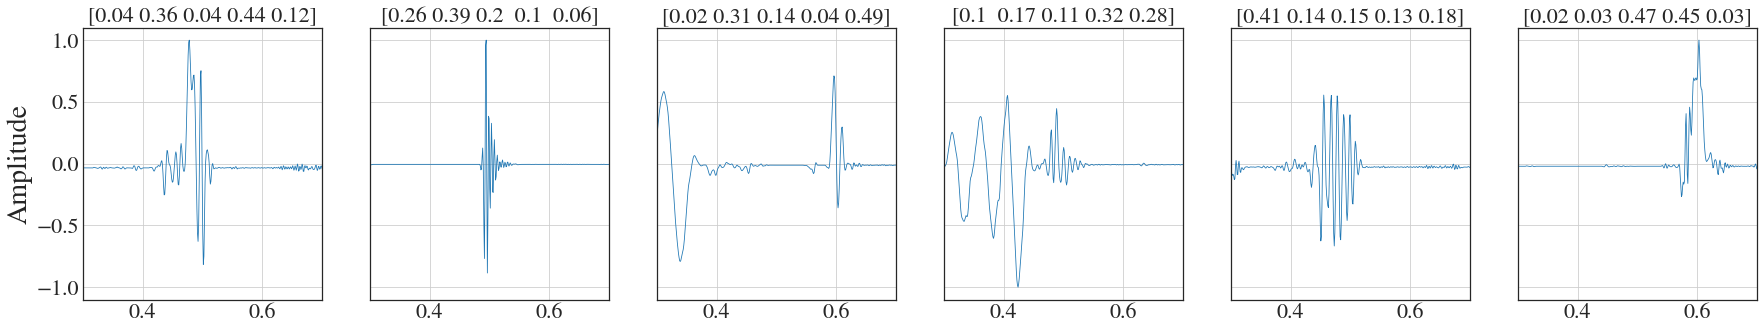
\includegraphics[width=\textwidth]{figures/generations/simplex_sample3.png}
    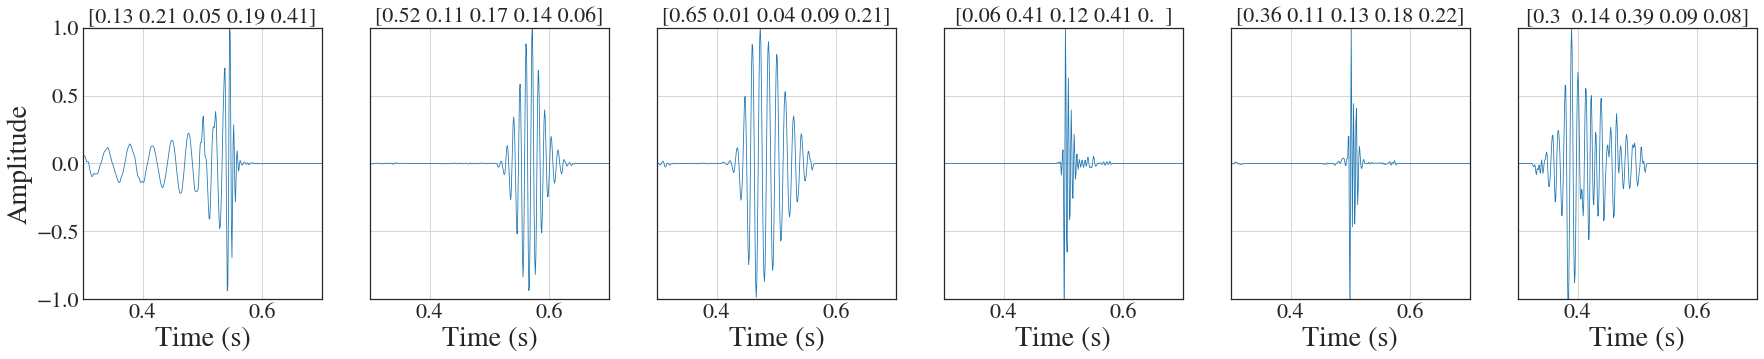
\includegraphics[width=\textwidth]{figures/generations/simplex_sample4.png}
    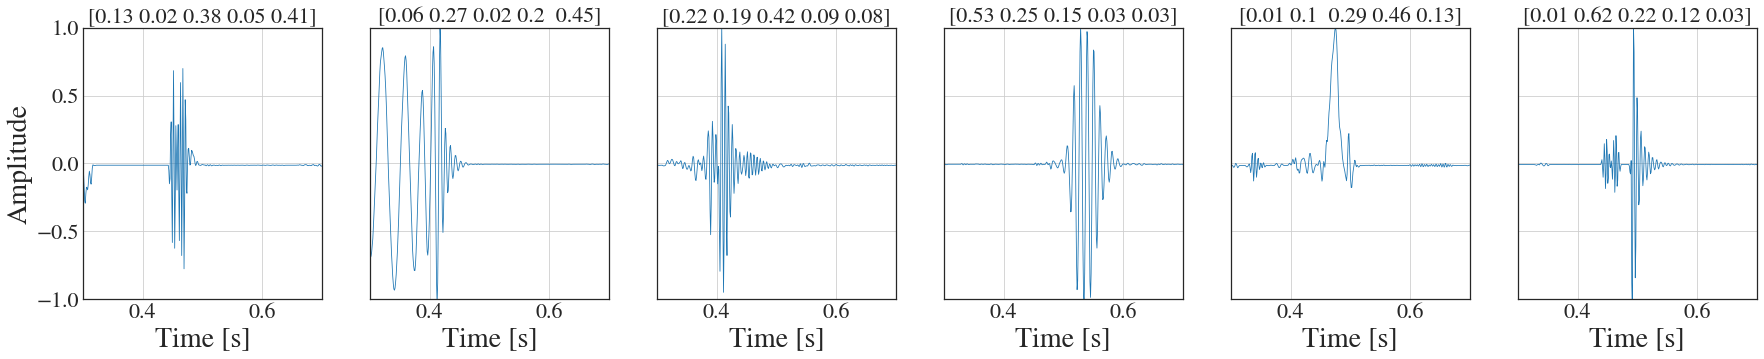
\includegraphics[width=\textwidth]{figures/generations/simplex_sample5.png}
    \caption{GAN generations where the class vectors are sampled from the \ndimensional{4} plane (simplex) intersecting all training classes. Latent space locations for all signals are taken randomly from a \ndimensional{100} Gaussian distribution and the signals are then re-scaled such that they have maximum absolute amplitude at unity. The class label for each generation is shown above each panel.}
    \label{fig:simplexd_samples}
\end{figure}

\begin{figure}
    \centering
    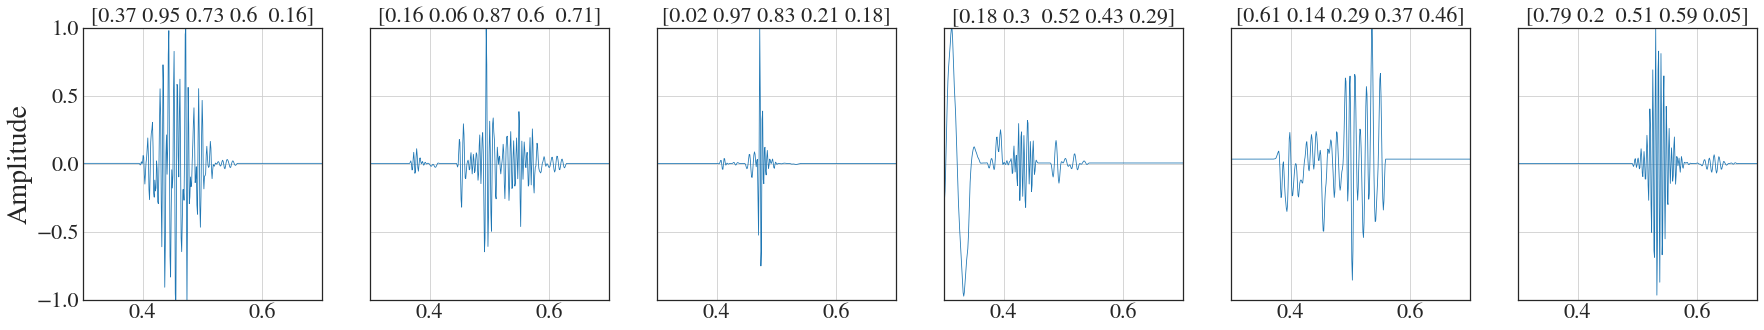
\includegraphics[width=\textwidth]{figures/generations/uniform_sample1.png}
    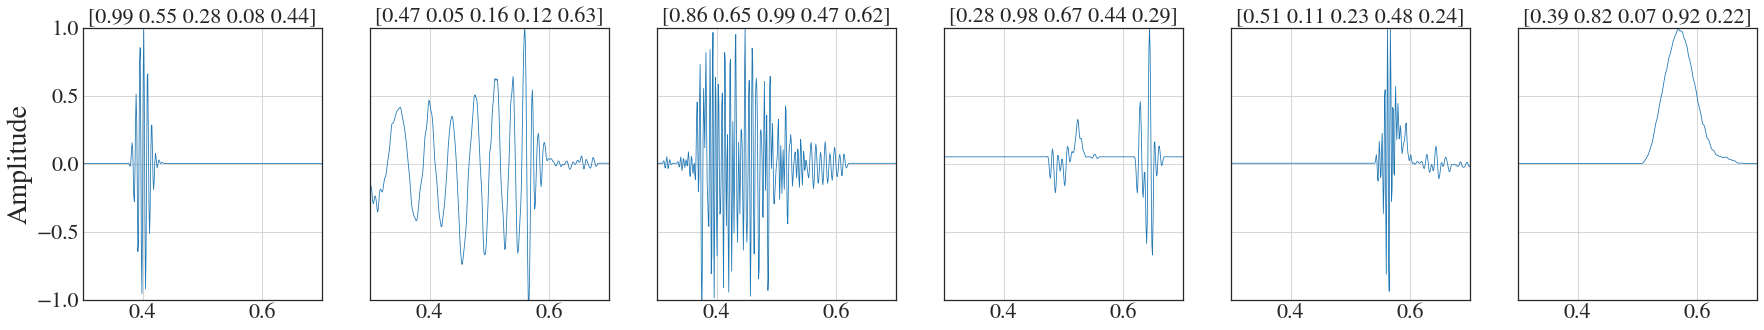
\includegraphics[width=\textwidth]{figures/generations/uniform_sample2.png}
    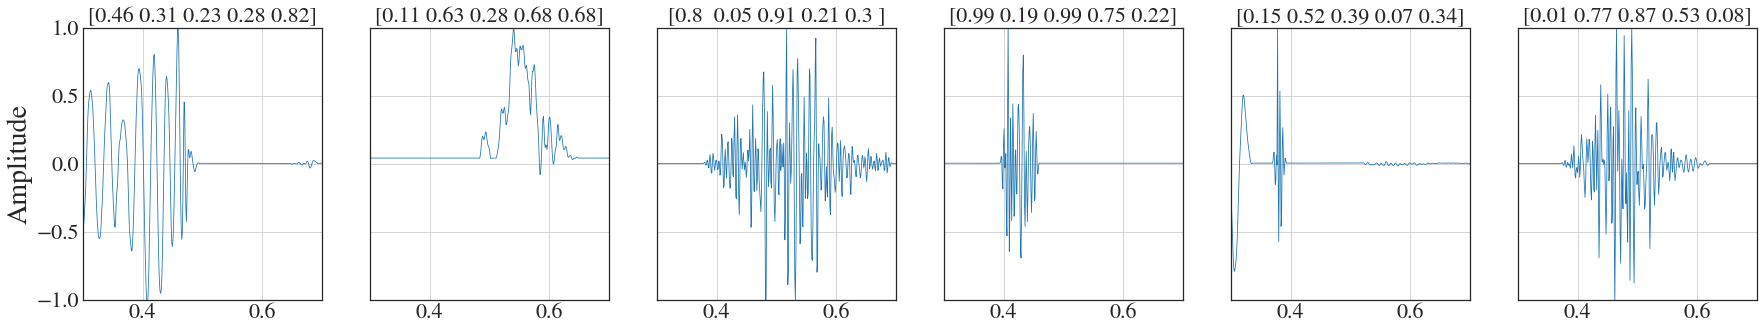
\includegraphics[width=\textwidth]{figures/generations/uniform_sample3.png}
    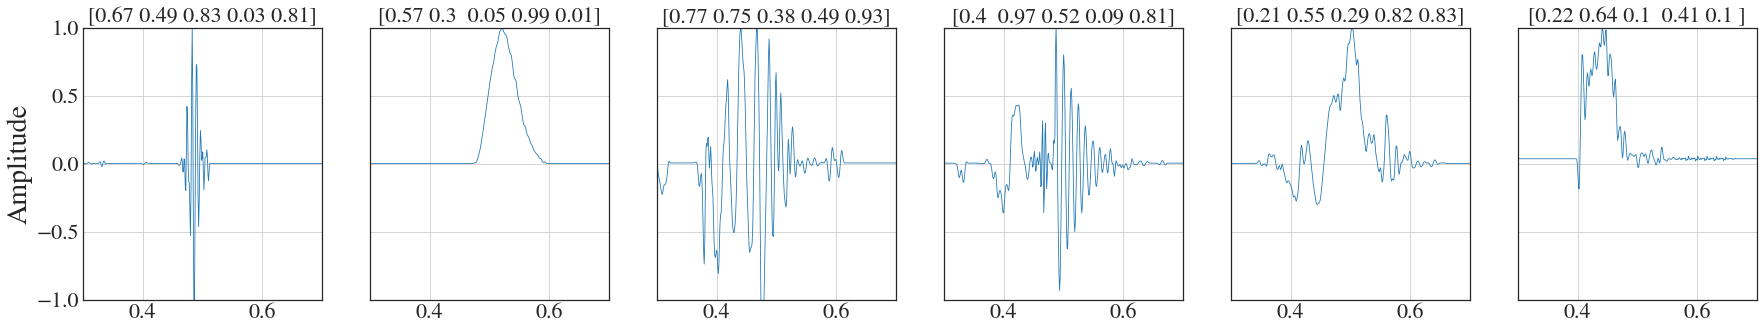
\includegraphics[width=\textwidth]{figures/generations/uniform_sample4.png}
    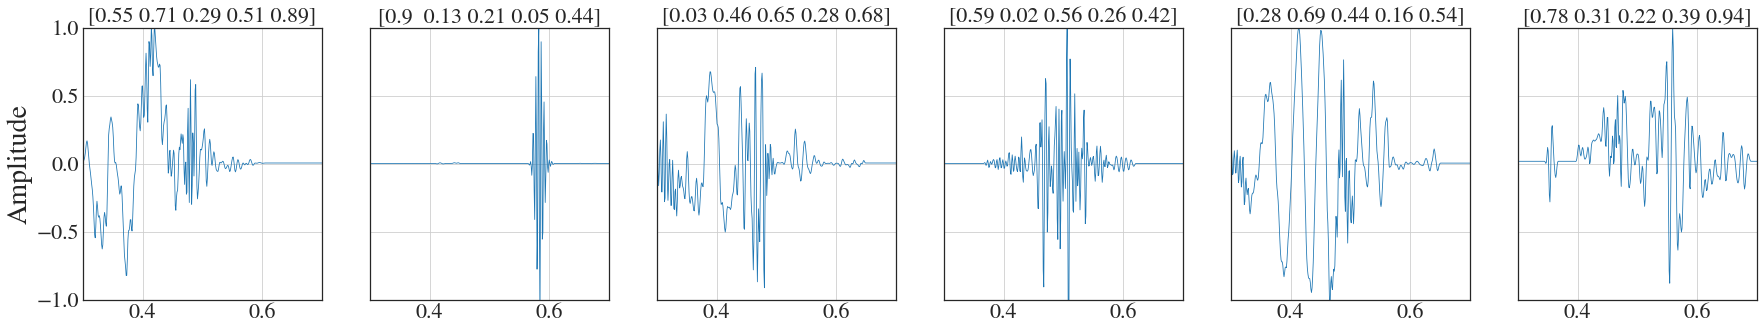
\includegraphics[width=\textwidth]{figures/generations/uniform_sample5.png}
    \caption{GAN generations where the class vectors are sampled uniformly in the hyper-cube class space. Latent space locations for all signals are taken randomly from a \ndimensional{100} Gaussian distribution and the signals are then re-scaled such that they have maximum absolute amplitude at unity. \michael{Same comment about y-axis labels}}
    \label{fig:uniform_samples}
\end{figure}

\section{CNN burst classifier} \label{cnn classifier}
In this section we develop a basic search analysis using a \ac{CNN} in order to compare the sensitivity of such a search to different \ac{GAN} generated waveforms in additive noise. We train a \ac{CNN} to perform simple classification and to distinguish between two classes: signals in additive Gaussian noise and Gaussian noise only. We are primarily interested in the relative sensitivity as a function of the types of waveforms used for training the network. We are also interested in how these differently trained networks perform when applied to data from waveform generations not used in the training process.

\subsection{Noisy datasets} 
We use three classes of waveforms: vertex, uniform, and simplex cases generated using our \ac{GAN} method. We then construct noisy time-series data from each waveform representing measurements from the 2 LIGO detector sites, Hanford (H1) and Livingston (L1). For each training set we generate $2\times 10^5$ signals and apply antenna responses and sky location dependent relative time delays using routines provided within LALsuite \cite{lalsuite}. The generated waveforms are used to represent the plus-polarisation component of signal only and the polarisation angles are drawn uniformly in the range $[0,2\pi]$ and sky positions are sampled isotropically. Time delays between detectors are computed relative to the Earth centre. All of the training data used is whitened using the Advanced LIGO design sensitivity \ac{PSD}\chris{add reference}, such that there is equal noise power at each frequency. Signal network \acp{SNR} is drawn uniformly in the range $[1,16]$ and is controlled by an amplitude scaling applied to the waveform. Each 1 second duration time-series input to the \ac{CNN} is represented by a \ndimensional{1} 1024 sample vector with 2 channels representing each detector. Example time-series from each detector for a single signal is shown in \cref{fig:cnn_training}. The network is trained to be able to identify whether or not a measurement contains a signal and therefore 50\% of the training data have time-series containing signals and 50\% have only noise. We randomly divide the data into the 3 standard sets (training, validation, and test data) where 40\% is used for training, 10\% used for validation, and 50\% is used for testing in order to achieve suitably low false-alarm rates. For the Uniform and Simplex datasets samples are drawn uniformly from their respective spaces. For the vertex data-set the 5 different vertex locations in class space are sampled with equal probability.  

\begin{figure}[ht!]
    \centering
    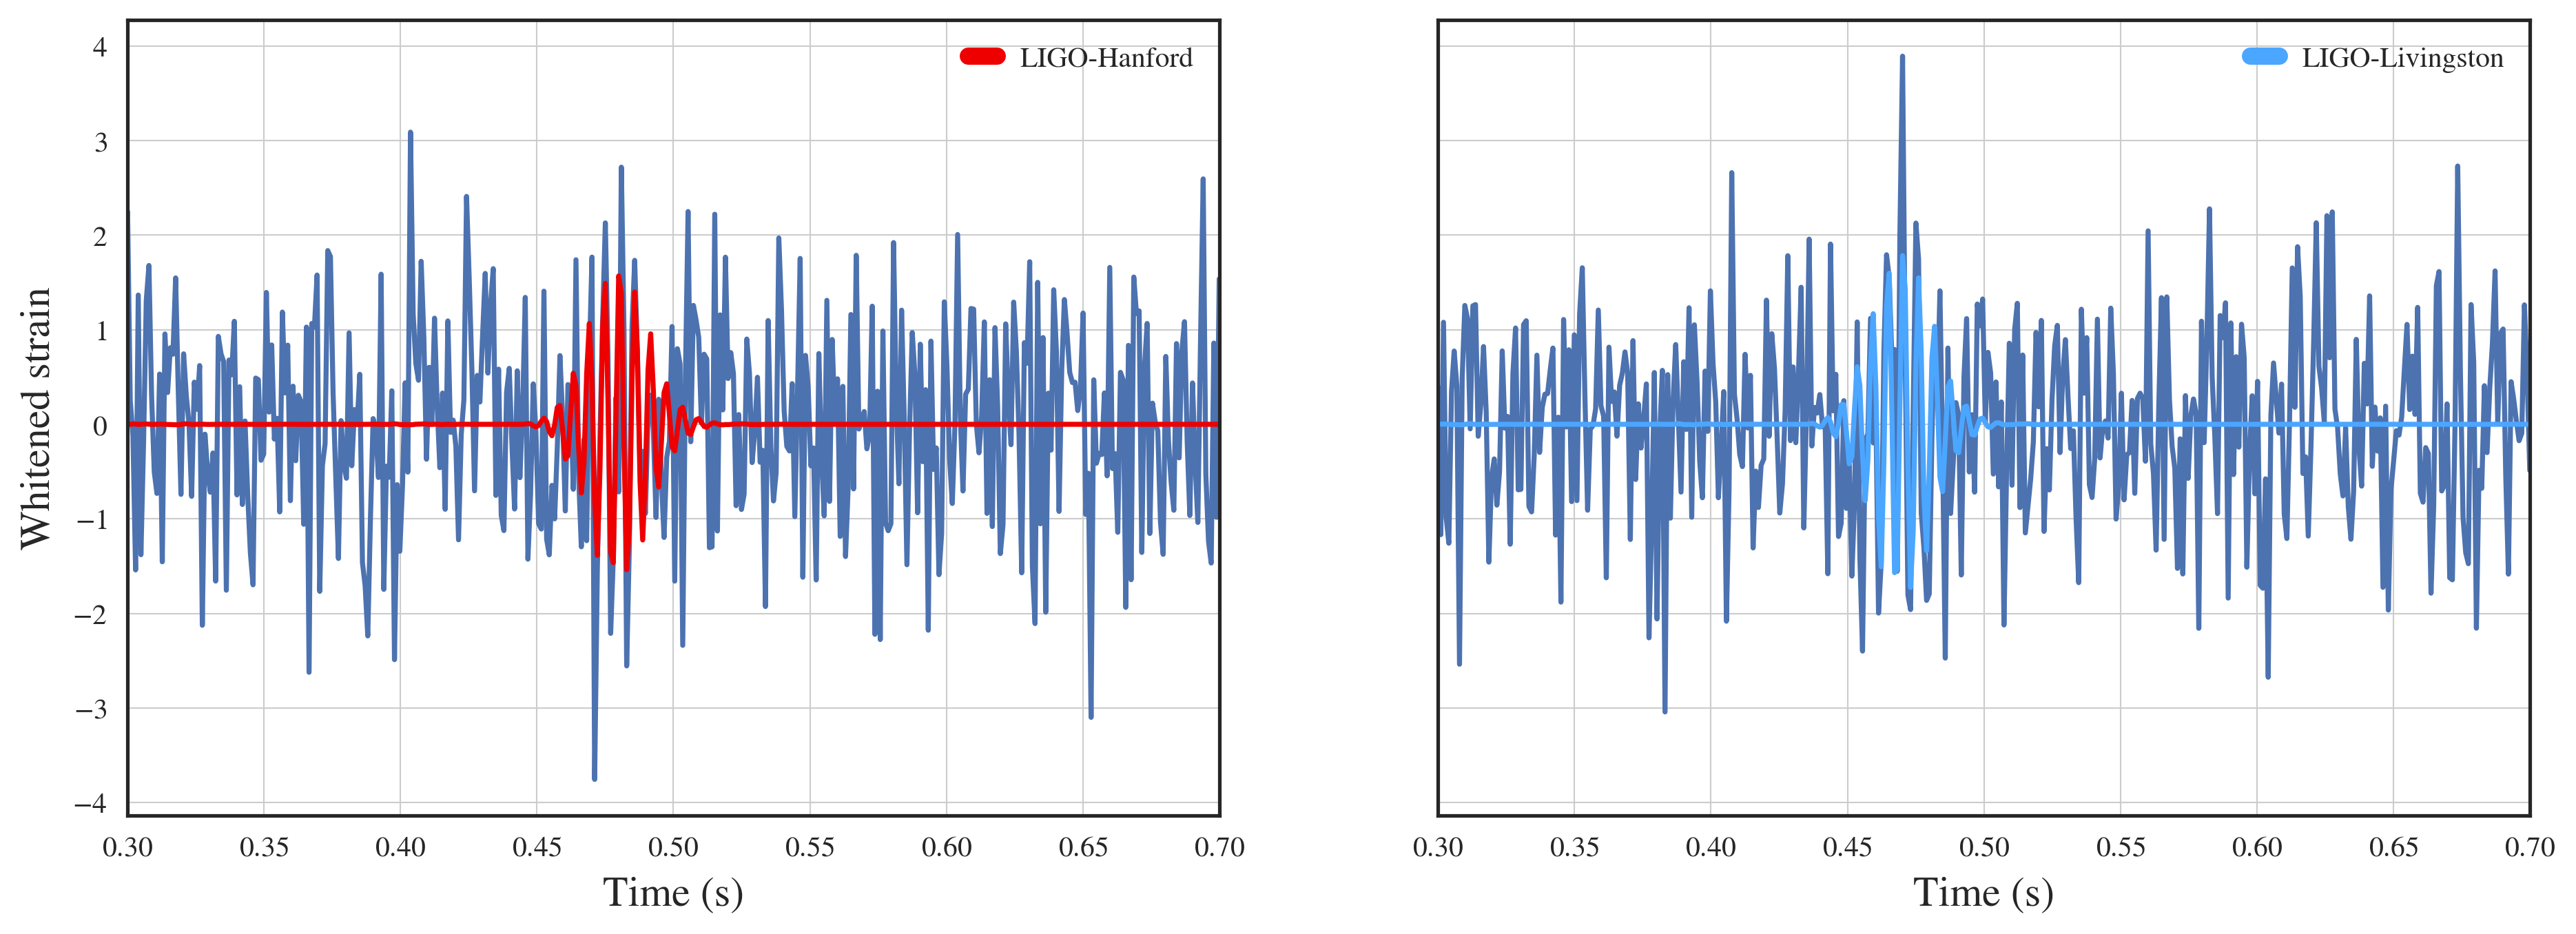
\includegraphics[width=\textwidth]{figures/SNR8.png}
    \caption{Example of \ac{CNN} training data showing a whitened noisy (dark blue) and noise-free (red, light blue) sine-Gaussian time-series as seen by Hanford (left) and Livingston (right) detectors. This signal has network $\text{SNR}=8$.}
     \label{fig:cnn_training}
\end{figure}

\subsection{CNN architecture}
In this approach the input to the \ac{CNN} are 1024 sample time-series (with 2 channels representing each detector output) which are passed through a series of 4 convolutional layers, onto two fully connected or ``Dense'' layers and finally to a single output neuron which represents the probability that a signal is present within the noise. We used dropout in the final dense layer and used a selection of different activation functions including the swish activation \cite{ramachandran2017searching} which improved overall performance and a sigmoid activation for the output layer. We used binary cross-entropy \cref{eqn:crossentropy} as the loss function and Adam as an optimizer with learning rate set to $10^{-3}$. In total we train three separate \acp{CNN} on the vertex, uniform and simplex datasets respectively. In each case the networks share the same architecture and hyperparameters which are defined in \cref{Tab:cnn_training_parms}.


\subsection{CNN results}
We now compare the \ac{CNN} results between the data-sets by first training three \acp{CNN} on the vertex, simplex, and uniform data-sets and then using these models to make predictions on the other testing data unseen during the network training process. In~\cref{fig:eff_curves} the top plot represents results from each trained network tested on the vertex data and shows that each model confidently classifies all data at 100\% for $\text{\ac{SNR}} >13$. At smaller \acp{SNR} the vertex and simplex perform similarly, however, the uniform data performs slightly worse. We would expect that when these models are tested on vertex data that everything should be classified at high \ac{SNR} as the vertex data is a subset of the uniform and vertex. The middle plot shows the results of the \acp{CNN} trained on simplex data.  As expected the simplex and vertex models recover 100\% detection at higher \acp{SNR} while the vertex trained model fails this test. This is explained when we consider that the simplex data is a subset of uniform while the vertex data is not. The final plot tests the models on uniform data and show again at high \acp{SNR} both simplex and uniform are 100\% detectable as a consequence of our previous subset argument. The vertex test is not fully detectable and further supports our premise that the vertex data, which is based on the modelled training data is distinguishable to both unmodelled datasets. 

The three tests shown previously show that the vertex model only manages full detection when tested on itself. The uniform model performs best in all cases and that it contains signals from the vertex and simplex samples, suggesting that this way of sampling the class space as input to the generator creates a good variety of unmodelled generations. 


\begin{comment}
\begin{itemize}
    \item vertex trained shows clear delineation from other two classes at \ac{SNR}$>$10. Good to show that they are different. But not all converge to 1.
    \item simplex trained leads in smaller \acp{SNR} but eventually all converge to 1
    \item uniform trained shows much similarity to simplex test set, still different from vertex. all converge to 1. makes sense if the vertex is a subset of the simplex and uniform classes. Also a sign that the \ac{GAN} likes to keep things as close to vertex as possible? 
\end{itemize}
\end{comment}

\begin{figure}[h!] % "[t!]" placement specifier just for this example
\centering
\begin{subfigure}{0.7\textwidth}
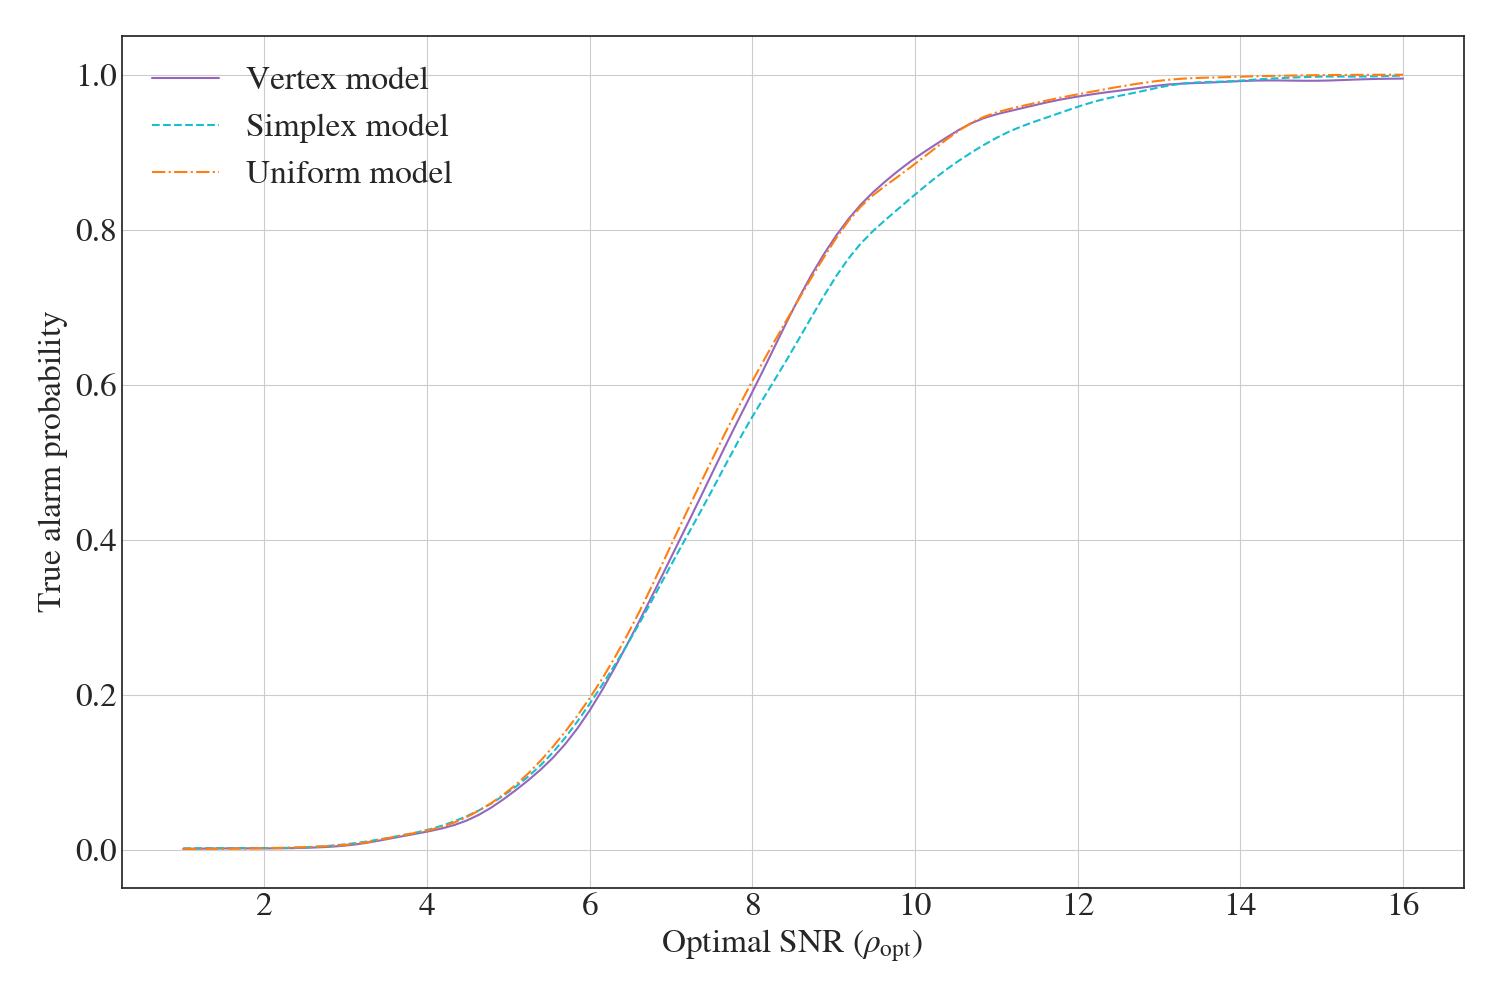
\includegraphics[width=\linewidth]{figures/efficiency_curve_vtest.png}
\end{subfigure}

\begin{subfigure}{0.7\textwidth}
\centering
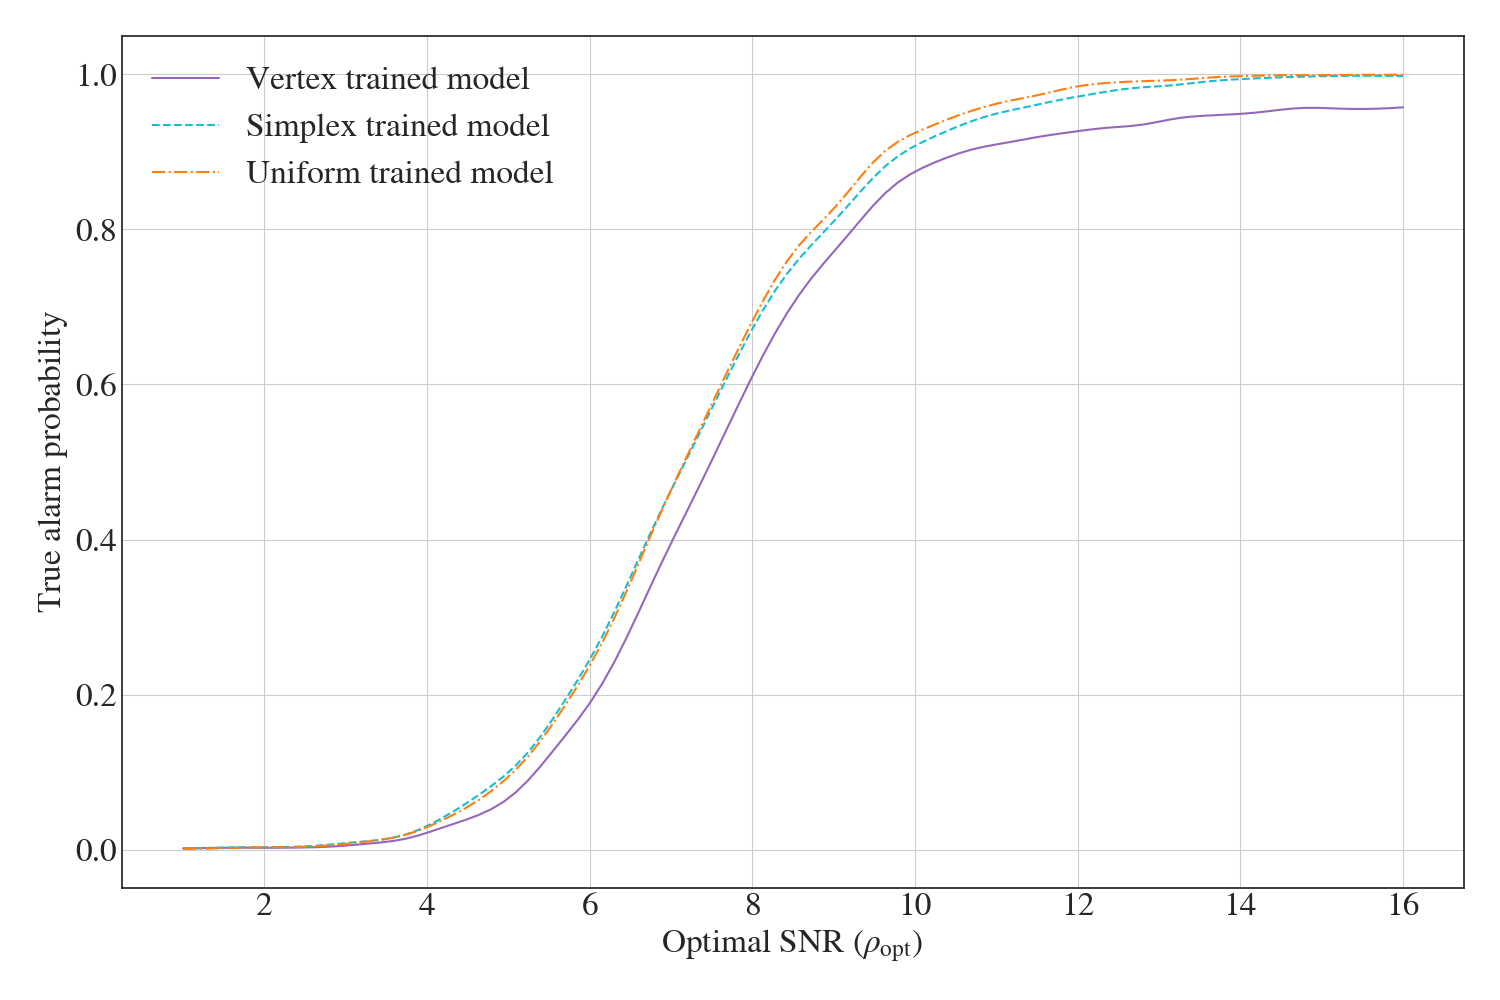
\includegraphics[width=\linewidth]{figures/efficiency_curve_stest.png}
\end{subfigure}

\begin{subfigure}{0.7\textwidth}
\centering
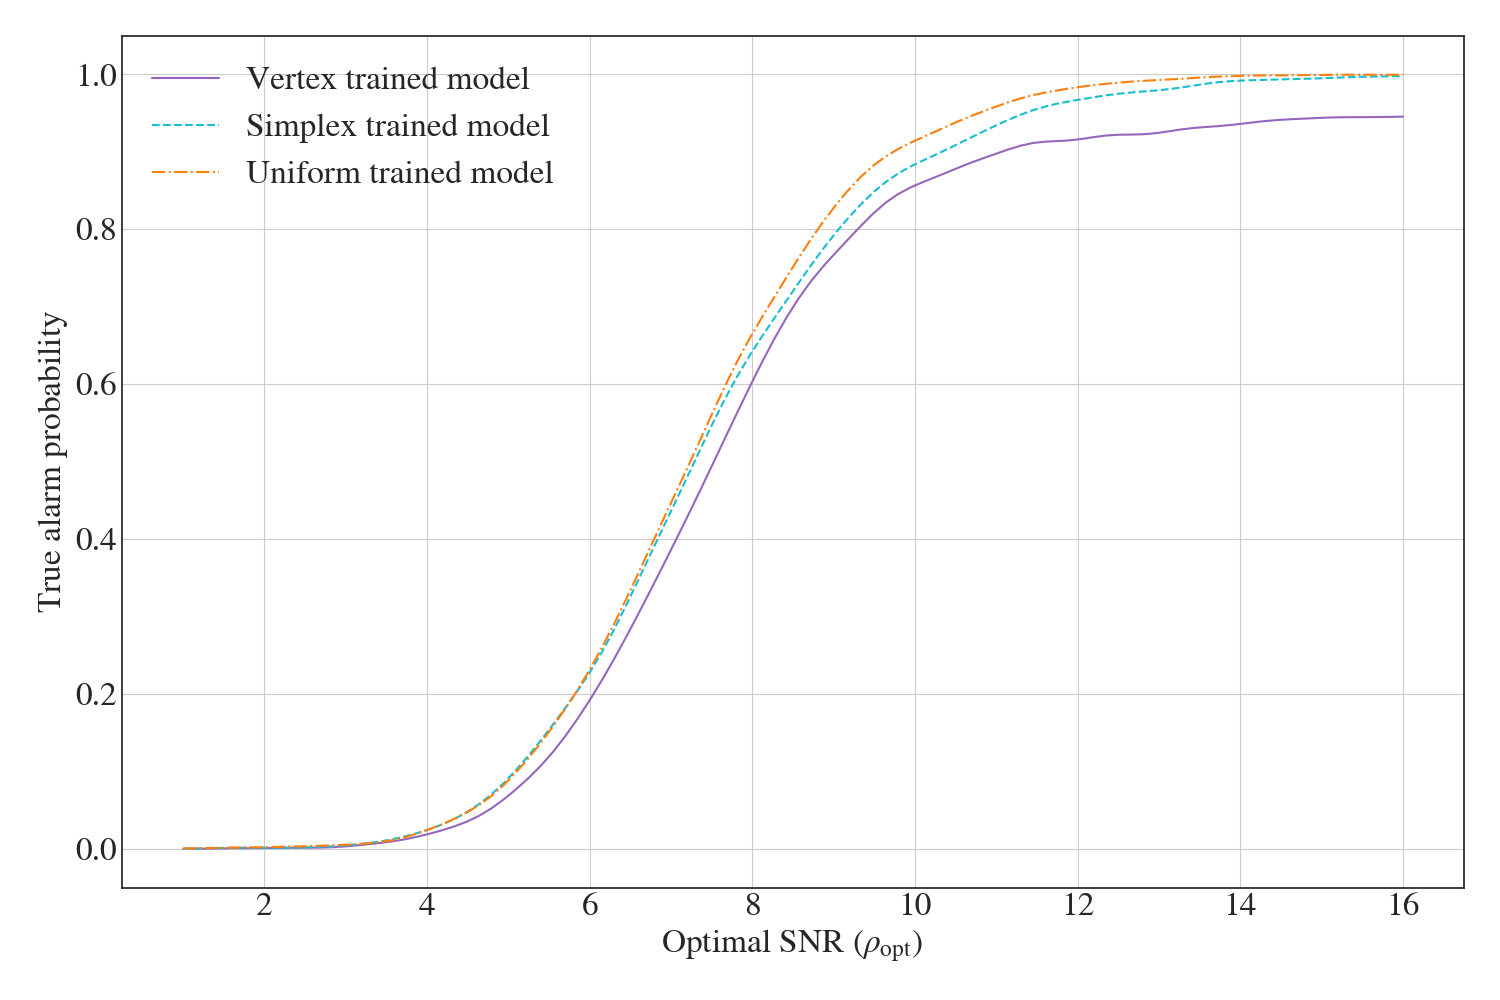
\includegraphics[width=\linewidth]{figures/efficiency_curve_utest.png}
\end{subfigure}

\caption{Efficiency curves comparing the performance of the \acp{CNN}. The true alarm probability is plotted as a function of the optimal \ac{SNR} of the signals. Each plot shows the performance of a \ac{CNN} trained on vertex, simplex and uniform datasets tested on vertex (top), simplex (middle), uniform (bottom). \michael{Maybe add a subcaption under each saying which dataset the models are tested on}}
\label{fig:eff_curves}
\end{figure}

%%%%%%%%%%%%%%%%%%%%%%%%%%%%%%%%%%%%%%%%%%%%%%%%%%%%%%%%%%%%%%%%%%%%%%%%%%%%%%
\section{Conclusions}\label{conclusions}
%%%%%%%%%%%%%%%%%%%%%%%%%%%%%%%%%%%%%%%%%%%%%%%%%%%%%%%%%%%%%%%%%%%%%%%%%%%%%%

% summary of the paper
%

In this work we present the potential of \acp{GAN} for
burst \ac{GW} generation. We have shown that \acp{GAN} have the ability to generate plausible time series burst data and present a novel approach to generating unmodelled waveforms. We have shown that CGANs are able distinguish between five distinct classes of burst like signals through conditional training which we can then utilise for targeted generations. 

We also show how our \ac{GAN} constructs smooth latent and class spaces during training and we explore these through interpolation showing smooth translations between classes and overall
waveform shape. Further, we showed targeted waveform generation by mixing classes in the class space through novel ways. We are able to produce new unmodelled waveform varieties vastly different from the training set and any known analytical method of generating these signals. Such waveforms are in demand in gravitational wave detection as they allow developers to test their search pipelines and other detection schemes.

We then considered three cases of unmodelled generated signals in Gaussian noise and trained a \ac{CNN} on those data. The resulting efficiency curves comparing the detection sensitivities of the \ac{CNN} as a function of \ac{SNR} of the waveforms showed that these signals were detectable in noise. Although the three datasets were similarly detectable there was some degree of separation between them.

In contrast to typical approaches in signal generation this is the first time a \ac{GAN} has been used for generating gravitational wave burst data. In the future, as development in \acp{GAN} and generative machine learning advances it is expected that we will gain greater control over target generation of features. 

Going forward it will also be important to extend our models to treat longer waveforms, higher sampling rates and conditioning on additional classes. One such class of interest would be ``glitch'' data. High amplitude short duration, peaks in the output of LIGO detectors that are internal sources of noise rather than of astrophysical origin. Using a \ac{GAN} to model these would aid in the understanding of these glitches and could help to remove them in order to get the cleanest data stream possible. 

Having the ability to quickly
generate new waveforms is essential to test current detection schemes and their
susceptibilty to unmodeled sources. We have shown that \acp{GAN} have the ability
to generate high fidelity waveforms which do not rely on large prior parameter space. Having banks of these
waveforms at hand can aid in our understand of the physics processes behind
these non-standard \ac{GW} emitters.  



\begin{comment}
\begin{itemize}
\item Summarise the paper
\item Dedicate a paragraph to each of the key results discussed in the previous
section
\item Have at least one paragraph on the future directions of this work
\item Conclude with a positive paragrpah about the potential uses and impact of
the approach.
\end{itemize}
\end{comment}

\section*{References}
\bibliography{references}

\clearpage

\appendix
\section{List of hyperparameters}

\begin{table}[hb]
\centering
\caption{The architecture and hyperparameters describing our \ac{GAN} consisting of discriminator and generator convolution neural networks. The discriminator casts the class input through a fully connected layer such that its dimensions match the signals input which it then concatenates channel-wise. This is then downsampled through four convolutional layers all activated by Leaky ReLU functions add drops half of the connections at the end of each of these layers. The vector is then flattened to one dimension before fully connecting to a single neuron and its output activated by sigmoid to represent the probability the signal came from the training set. The generator concatenates the latent and class input vectors which is fed to a fully connected layer. This layer is then upsampled by four tranposed convolutions. Batch normalisation is applied to the output of the first layer and all convolutional layers are activated by ReLU with the exception of the final layer which is Linear. Finally, the extra dimension introduced for the convolution is removed. \michael{You say 500 epochs in the test but 100 here, not sure which is right. Also could include learning rate with tyhe optimiser}}
%\footnotesize
\begin{tabular*}{\textwidth}{c @{\extracolsep{\fill}} c c c c c c}
\br
\mr
%\hline
&& Discriminator &&& \\
\mr
Operation & Output shape & Kernel size & Stride & Dropout & Activation \\
Class Input & (5) & - & - & 0  & - \\
Dense & (1024) & - & - & 0 & - \\
Signal Input & (1024) & - & - & 0 &  - \\
Concatenate & (1024, 2) & - & - & 0 &  - \\
Convolutional & (512, 64) & 14 & 2 & 0.5 & Leaky ReLU \\
Convolutional & (256, 128) & 14 & 2 & 0.5 &  Leaky ReLU \\
Convolutional & (128, 256) & 14 & 2 & 0.5 & Leaky ReLU \\
Convolutional & (64, 512) & 14 & 2 & 0.5 &  Leaky ReLU \\
Flatten & (32768) & - & - & 0 &  - \\
Dense & (1) & - & - & 0 & sigmoid \\
\mr
&& Generator &&& \\
\mr
Operation & Output shape & Kernel size & Stride & BN & Activation \\
Class Input & (5) & - & - & \ding{55}  & - \\
Latent Input  & (100) & - & - & \ding{55} & - \\
Concatenate & (105) & - & - & \ding{55} &  - \\
Dense & (32768) & - & - & \ding{55} &  ReLu \\
Reshape & (64, 512) & - & - & \ding{55} & - \\
Transposed Conv & (128, 256) & 18 & 2 & \ding{51} & ReLU \\
Transposed Conv & (256, 128) & 18 & 2 & \ding{55} &  ReLU \\
Transposed Conv & (512, 264) & 18 & 2 & \ding{55} & ReLU \\
Transposed Conv & (1024, 1) & 18 & 2 & \ding{55} & Linear \\
Reshape & (1024) & - & - & \ding{55} & - \\
\end{tabular*}
\begin{tabular*}{\textwidth}{@{} l l l l l l}
\mr
 Optimizer & Adam($\alpha$ = 0.0002, $\beta_{1}$ = 0.5) \\
 Batch size & 512  \\
 Epochs & 100  \\
 Loss & Binary cross-entropy \\
 \mr
 \br
\end{tabular*}\\
\label{Tab:gan_training_parms}
\end{table}

\begin{table}[hb]
\centering
\caption{The architecture and hyperparameters describing our CNN consists of four convolutional layers followed by two dense layers. The convolutional and dense layers are activated by the swish function \cite{ramachandran2017searching} and dropout is applied, while the final layer uses the sigmoid activation. The network is trained by minimising the binary cross entropy and optimised with Adam with learning rate $10^{-3}$. We train for 100 epochs with a batch size of 1000.}
%\footnotesize
\begin{tabular*}{\textwidth}{c @{\extracolsep{\fill}} c c c c c c}
\br
%\hline
Operation & Output shape & Kernel size & Stride & Dropout & Activation \\
\mr
Input & (1024, 2) & -  & - & - & - \\
Convolutional & (512, 8) & 5 & 2 & 0 & Swish  \\
Convolutional & (256, 8) & 5 & 2 & 0 & Swish  \\
Convolutional & (128, 8) & 5 & 2 & 0 & Swish  \\
Convolutional & (64, 8) & 5 & 2 & 0 & Swish  \\
Dense & (100) & 100 & - & 0.2 & Swish  \\
Dense & (1) & 1 & - & 0 & sigmoid \\
\end{tabular*}\\
\begin{tabular*}{\textwidth}{@{}l l l l l l}
\mr
Optimizer & Adam($\alpha$ = 0.001, $\beta_{1}$ = 0.5) & & & & \\
Batch size & 1000 & & & & \\
Epochs & 100 & & & & \\
Loss & Binary cross-entropy & & & & \\
 \br
\end{tabular*}\\
\label{Tab:cnn_training_parms}
\end{table}

\section{Many more generated examples}
~\chris{do we still need this?}

\end{document}
